\section{Auswertung}

Im Folgenden wird der große Block der PLL, bestehend aus VCO, Phasendetektor und Schleifenfilter, nach ihrer Funktionsweise untersucht. In diesem Abschnitt befinden sich auch die Herleitungen für die Dimensionierung der verwendeten Bauteile in diesen Blöcken. Am Ende wird die Funktionsweise der zusammengebauten PLL genauer untersucht.

\subsection{Dreieck-Rechteck-VCO}

Als erstes wird der Aufbau und die Funktionsweise des Dreieck-Rechteck-VCOs genauer untersucht. Der Oszillator,der im letzten Laborverusch aufgebaut wurde, wurde durch zwei Emitterfolger ergänzt.(\ref{fig:VCO_Schaltung} Diese Schaltung schaltet zwischen einer einstellbaren Steuerspannung und ihrem Komplementärsignal um, welche zuvor vom Spannungsfolger und dem invertierenden Verstärker erzeugt wurden.

Die Kombination aus Emitterfolger und Widerstand $R_3$ ist äquivalent zu einer umschaltbaren Stromquelle, die abwechselnd den Kondensator des Integrators lädt und entlädt. Bei einer Änderung des Stroms dieser Quelle und somit der Spannung über dem Widerstand verändert sich die Ladezeit des Kondensators und damit die Frequenz des gesamten Oszillators. Als Konsequenz stellt sich am Ausgang des Schmitttriggers ein steuerspannungsabhängiges Rechtecksignal ein, das für die PLL genutzt werden kann.
\begin{figure}[H]
  \centering
  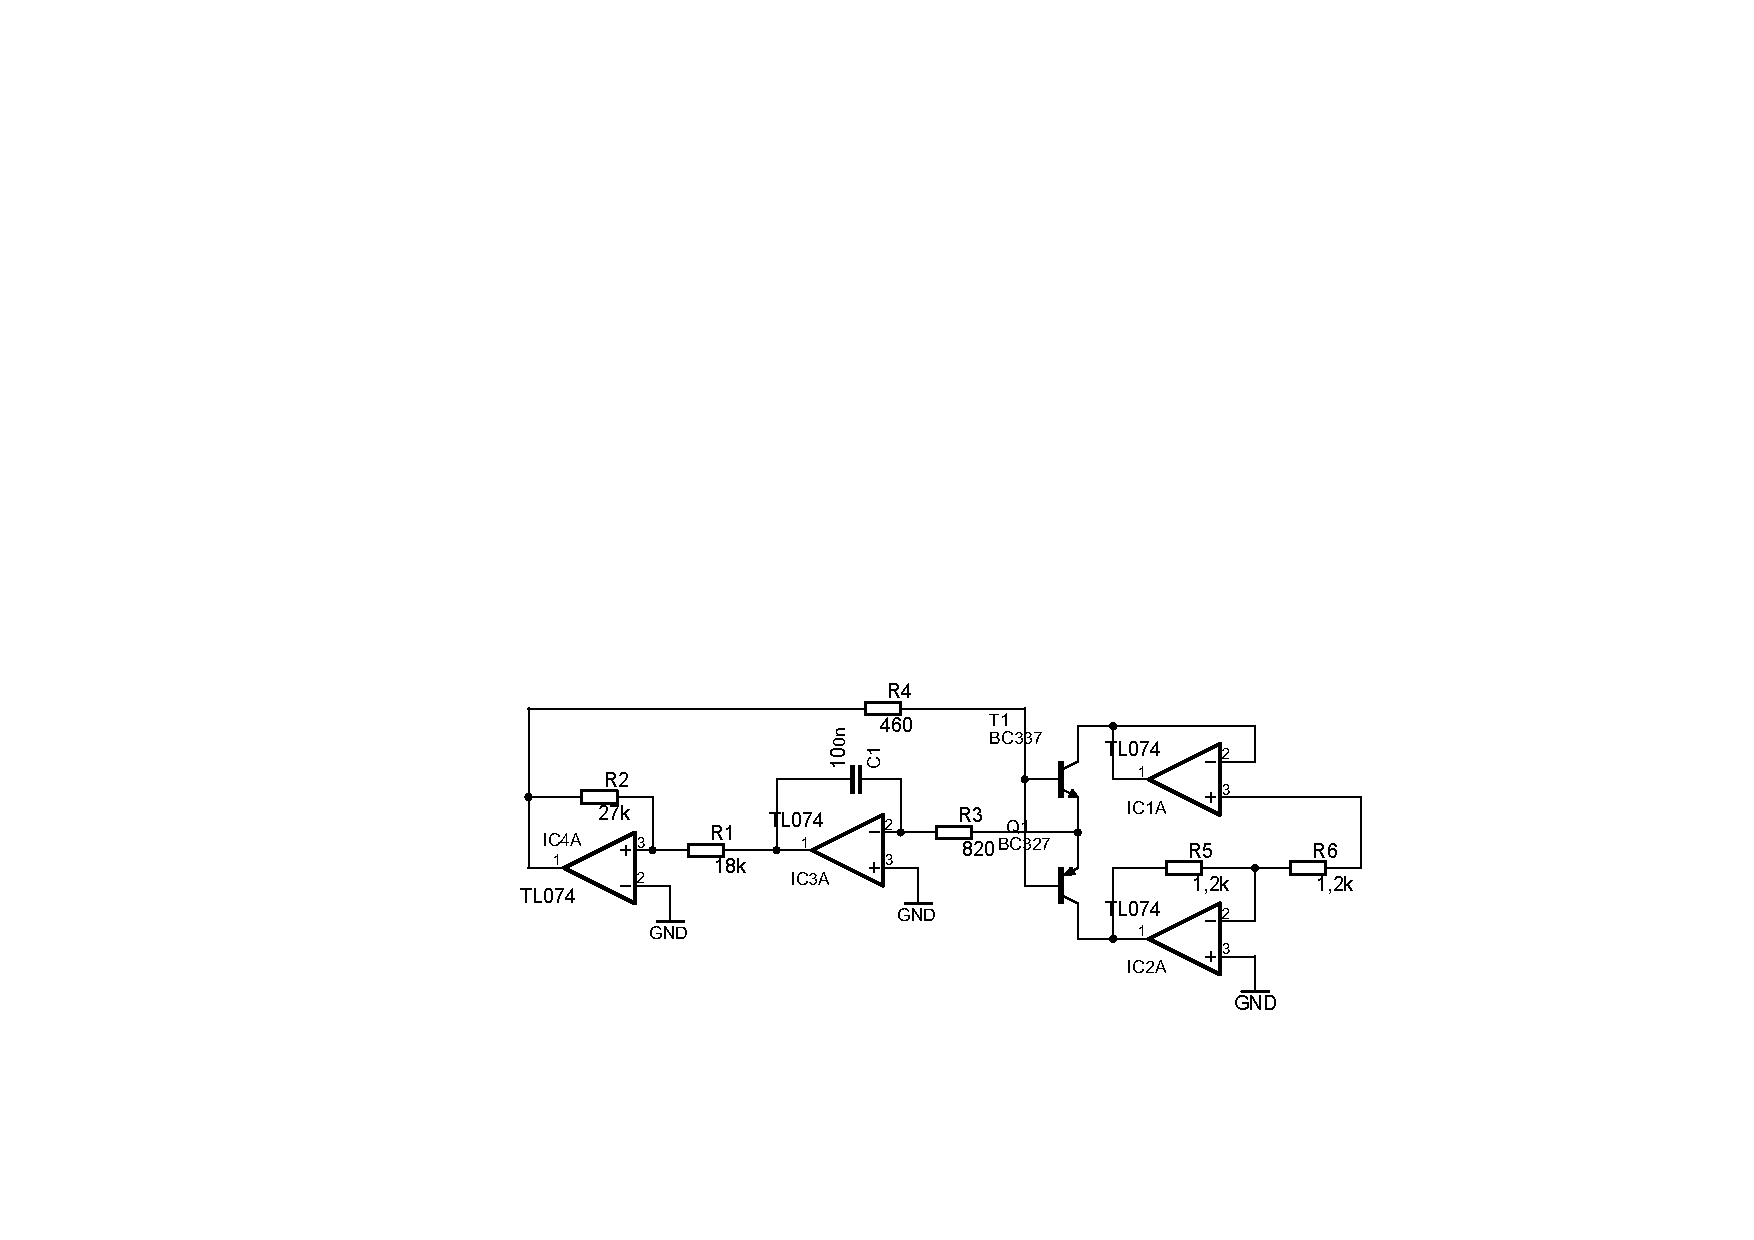
\includegraphics[width=1\linewidth]{Elektronik-Laborprotokoll_PLL/Abbildungen/VCO_Schaltung.pdf}
  \caption{Dreieck-Rechteck-VCO (Schaltplan)}
  \label{fig:VCO_Schaltung}
\end{figure}


%Dreieck-Rechteck-Oszillator aufzubauen. Dafür wird der Ausgang eines nichtinvertierenden Schmitt-Triggers an den Eingang eines invertierenden Integrator angeschlossen. Ebenfalls wird der Ausgang des invertierenden Integrator mit dem Eingang des nichtinvertierenden Schmitt-Triggers  verbunden.
%Schreibst du das fertig? ODder hatte ich das geschrieben?

\subsubsection{Dimensionierung des Schmitt-Triggers}

\begin{figure}[H]
    \centering
\begin{circuitikz}[european]
    \ctikzset{bipoles/length=1cm}
    
    \draw
    (0,0) node[op amp,yscale=-1] (opamp) {};
    
    \draw (opamp.+) to[R, european resistor, l=$R_1$] (-2, 0.35) -- (-3, 0.35) node[ocirc]{};
    
    \draw [-latex] ([yshift=-2mm] -3,0.35)--(-3,-1.35) node[midway,left] {$U_e$} ; 
   
 % Zeichne C   
    \draw (opamp.+) to[short,*-] ++(0,0.75) coordinate (leftD) to[short,-*](leftD)
    to[R, l=$R_2$] (leftD -| opamp.out) to[short,-*](leftD -| opamp.out) ;

    \draw [-latex] ([yshift=-2mm] opamp.out)--(0.85,-1.35) node[midway,left] {$U_a$}; 
    
    \draw (0.85,-1.45) node[ocirc]{} to(0.85,-1.5) node[ground]{};
    \draw (-3,-1.45)node[ocirc]{}to(-3,-1.5) node[ground]{};

   \draw (opamp.out)--(2,0) node[ocirc]{};
% Zeichne R2
   \draw (leftD -| opamp.out) to[short,*-](leftD -| opamp.out) to ( opamp.out);

    \draw (opamp.-) -- (-1,-0.35) to (-1,-1.5) node[ground]{};
  
\end{circuitikz}
  \caption{Schmitt-Trigger}
    \label{fig:schmitt}
\end{figure}

Gegeben sind die Versorgungsspannung \( V_{CC}=\SI{12}{\volt} \) und die Schaltschwellen eines nicht-invertierenden Schmitt-Triggers \( U_{E,ON} = \frac{2\cdot V_{CC}}{3} \) und \( U_{E,OFF} = -\frac{2\cdot V_{CC}}{3} \). Die Widerstände \( R_1 \) und \( R_2 \) sollen bestimmt werden. Die Beziehungen zwischen den Schaltschwellen und den Widerständen sind:

\begin{align*}
  U_{E,ON}=-\frac{R_1}{R_2}\cdot U_{A,min}
\end{align*}
Dabei ist \( U_{A,min} \) die minimale Ausgangsspannung des Operationsverstärkers, die durch die Verbindung der negativen Versorgungsspannung (VSS) mit dem Ausgang bestimmt wird. \cite[S.~17, Gl.~2.3]{Skript}:

Wird der Wert von $U_{E,ON}$ eingesetzt. Und sei $U_{A,min}=-V_{CC}$ .
%Eingesetzt wird
\begin{align*}
 \frac{2}{3}\cdot V_{CC}=-\frac{R_1}{R_2}\cdot (-V_{CC})
\end{align*}

Durch die Umformung folgt:

\begin{align*}
2R_2=3R_1
\end{align*}

und 
\begin{align*}
R_2=1,5 \cdot R_1
\end{align*}

Freiwillig ausgewählt anhand verfügbarer Wiederstände ist $R_1$=\SI{18}{\kilo\ohm}. Daraus folgt für $R_2$:

\begin{align*}
R_2=1,5 \cdot \SI{18}{\kilo\ohm} =\SI{27}{\kilo\ohm}
\end{align*}

\subsubsection{Dimensionierung des Integrators}

\begin{figure}[H]
    \centering
\begin{circuitikz}[european]
    \ctikzset{bipoles/length=1cm}
    \draw
    (0,0) node[op amp,yscale=1] (opamp) {};
    
    \draw (opamp.-) to[R, european resistor, l=$R_3$] (-2, 0.35) -- (-3, 0.35) node[ocirc]{};
    
    \draw [-latex] ([yshift=-2mm] -3,0.35)--(-3,-1.35) node[midway,left] {$U_e$} ; 
   
 % Zeichne C   
    \draw (opamp.-) to[short,*-] ++(0,0.75) coordinate (leftD) to[short,-*](leftD)
    to[C, l=$C_1$] (leftD -| opamp.out) to[short,-*](leftD -| opamp.out) ;

    \draw [-latex] ([yshift=-2mm] opamp.out)--(0.85,-1.35) node[midway,left] {$U_a$}; 
    
    \draw (0.85,-1.45) node[ocirc]{} to(0.85,-1.5) node[ground]{};
    \draw (-3,-1.45)node[ocirc]{}to(-3,-1.5) node[ground]{};

   \draw (opamp.out)--(2,0) node[ocirc]{};
% Zeichne R2
   \draw (leftD -| opamp.out) to[short,*-](leftD -| opamp.out) to ( opamp.out);

    \draw (opamp.+) -- (-1,-0.35) to (-1,-1.5) node[ground]{};
\end{circuitikz}
  \caption{Integrator}
    \label{fig:Integrator}
\end{figure}

Die maximale Frequenz des VCOs soll \SI{2}{\kilo\hertz} betragen. Im invertierenden Integrator ist ein Kondensator $C_1$=\SI{100}{\nano\farad} zu verwenden. Es soll der Widerstand $R_3$ dimensioniert werden.
 
Bei dem Integrator wird der Eingangstrom über eine bestimmte Zeitdauer $t$ integriert. Dabei wird angenommen, dass der Eingangsstrom $I_E$ während dieser Zeit konstant ist. Es gilt:

\begin{equation}
\label{eq:U_A_pp}
U_{A,pp} = U_{C_{\max{}}}-U_{C_{\min{}}}=\frac{1}{C} \cdot \int_{t_0}^{t_0+t} I_E , d\overline{t} = \frac{1}{C} \cdot I_E \cdot t
\end{equation}


Unter Verwendung des Ohmschen Gesetzes lässt sich der Eingangsstrom $I_E$ wie folgt berechnen:

\begin{equation}
\label{eq:Integrator_I_E}
    I_E=\frac{U_E}{R_E}
\end{equation}

Durch die Einsetzung der Gleichung \ref{eq:Integrator_I_E} in die Gleichung \ref{eq:U_A_pp} folgt:

\begin{equation*}
    U_{A,pp}=\frac{1}{C}\cdot \frac{U_E}{R_E} \cdot t
\end{equation*}

Der Integrator ist an den Schmitt-Trigger angeschlossen. Wenn die Ausgangsspannung des Integrators $U_A$ die Schaltschwelle des Schmitt-Triggers überschreitet, wechselt der Schmitt-Trigger zwischen den beiden Pegeln hin und her. Da die Schaltschwelle bei $\frac{2}{3} \cdot V_{CC}$ liegt, muss die Spitze der Dreieckschwingung ebenfalls $\frac{2}{3} \cdot V_{CC}$ betragen. Analog dazu beträgt das Minimum der Dreieckschwingung $-\frac{2}{3} \cdot V_{CC}$. Folglich ergibt sich für die Spitze-zu-Spitze-Spannung der Dreieckschwingung:

\begin{equation*}
U_{A,pp} =\frac{2}{3} \cdot V_{CC}-(-\frac{2}{3} \cdot V_{CC})=\frac{4}{3} \cdot V_{CC}
\end{equation*}

Mit Hilfe der Gleichung \ref{eq:U_A_pp} und unter Berücksichtigung der Periodendauer $t$ lässt sich nun die folgende Beziehung aufstellen:
    
\begin{equation*}
\frac{4}{3} \cdot V_{CC} = \frac{1}{C} \cdot \frac{U_E}{R_E} \cdot t
\end{equation*}
Da der Tastgrad des Rechtecksignals bei D=\SI{50}{\percent} liegt, folgt durch die Gleichung $t=\frac{T}{2}$:
\begin{equation*}
    \frac{4}{3}\cdot V_{CC}=\frac{1}{C}\cdot \frac{U_E}{R_E} \cdot \frac{T}{2}
\end{equation*}
Durch die Gleichung $f=\frac{1}{T}$ folgt:
\begin{equation*}
    \frac{4}{3}\cdot V_{CC}=\frac{1}{C}\cdot \frac{U_E}{R_E} \cdot \frac{1}{2f}
\end{equation*}
Durch die Umformung nach $R_E$ folgt:
\begin{equation*}
  R_E=\frac{U_E}{\frac{4}{3}\cdot V_{CC} \cdot C \cdot 2f}
\end{equation*}
Durch die Einsetzung der Werte folgt:
\begin{equation*}
 R_3=R_E=\frac{\SI{5}{\volt}}{\frac{4}{3}\cdot \SI{12}{\volt} \cdot \SI{100}{\nano\farad} \cdot 2 \cdot \SI{2}{\kilo\hertz}}=\SI{781,25}{\ohm}
\end{equation*}


Als nächster Wert für den berechneten Widerstand wird ein Wert aus der E12-Widerstandsreihe ausgewählt, sodass $R_3$=\SI{820}{\ohm} beträgt. 


%Finde hier Unterabschnitt
\subsubsection{Darstellung der Signale}
Bei unseren Messungen haben wir zwei Signale betrachtet: das Ausgangssignal des Schmitt-Triggers, welches eine Rechteckwelle ist, und das Ausgangssignal des Integrators. Aufgrund der Rechteckwellenform des Eingangssignals wird dieses vom Integrator in eine Dreieckschwingung umgewandelt. 

Die Abbildung \ref{fig:VCO_5Volt} zeigt die aufgebaute Dreieck-Rechteck-VCO.

\begin{figure}[H]
  \centering
  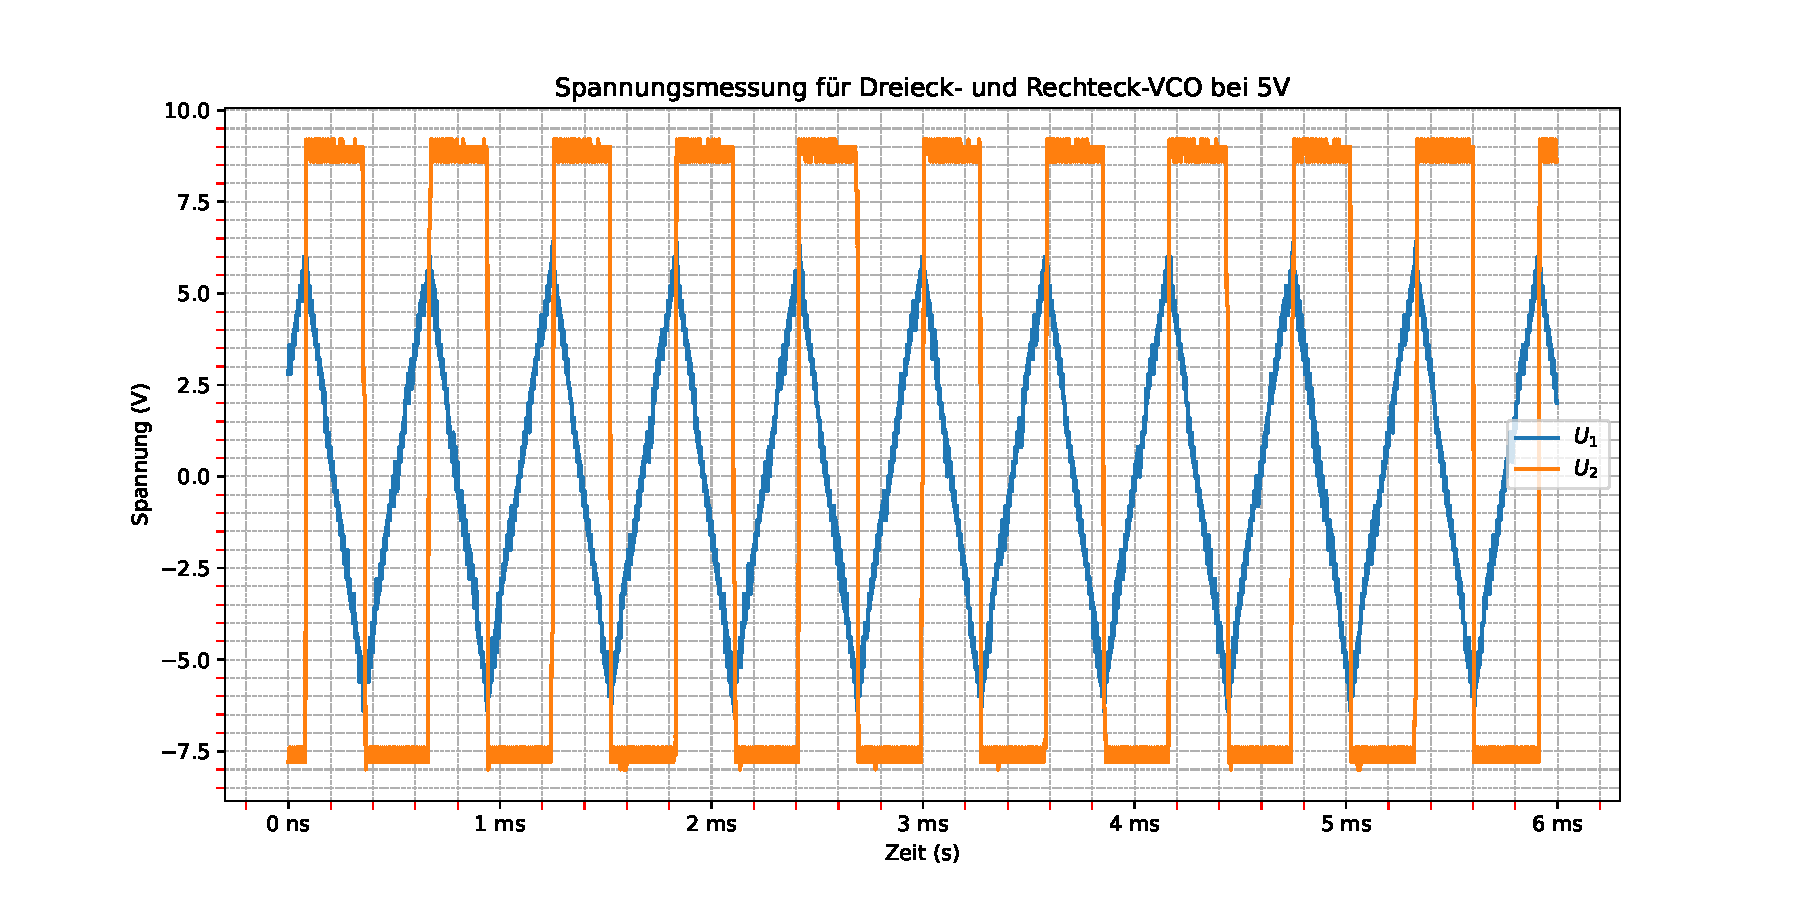
\includegraphics[width=0.8\linewidth]{Elektronik-Laborprotokoll_PLL/Plots/VCO_5V.pdf}
  \caption{Gemessen-VCO bei einer Eingangsspannung von \SI{5}{\volt}}
  \label{fig:VCO_5Volt}
\end{figure}

Die Abbildung \ref{fig:VCO_5Volt_Simulation} zeigt die simulierte Dreieck-Rechteck-VCO.

\begin{figure}[H]
  \centering
  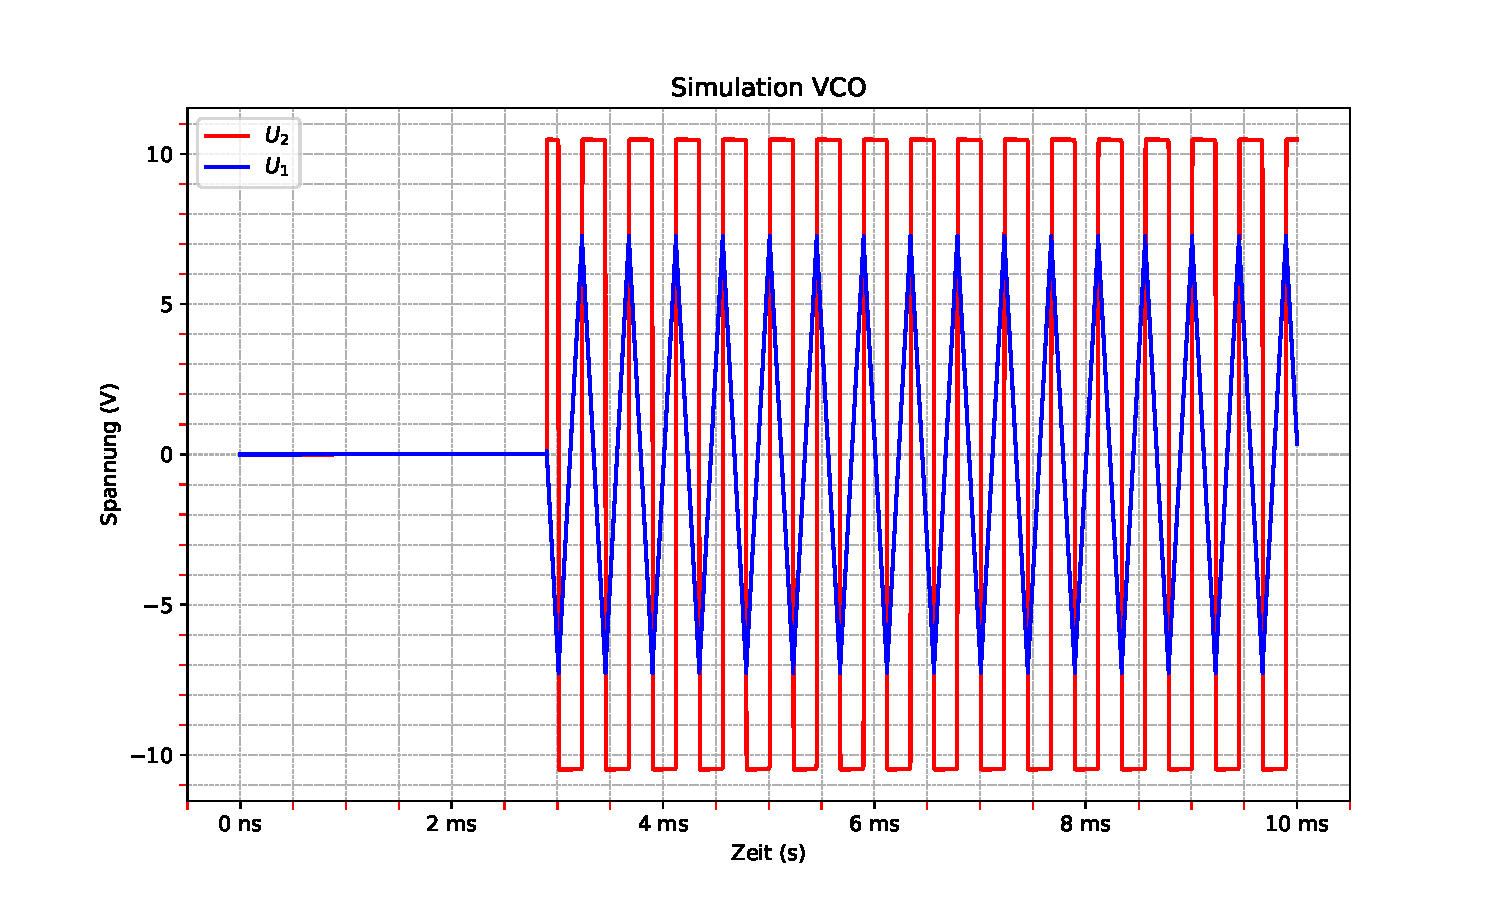
\includegraphics[width=0.8\linewidth]{Elektronik-Laborprotokoll_PLL/Plots/simulation-vco-5V.pdf}
  \caption{Simulation-VCO bei einer Eingangsspannung von \SI{5}{\volt}}
  \label{fig:VCO_5Volt_Simulation}
\end{figure}

\subsubsection{Kennlinie der Steuerspannung und der Ausgangsfrequenz}


In der Tabelle \ref{tab:VCO_Kennlinie_gemessen} sind die Frequenzen als Ausgangsgröße in Abhängigkeit der Eingangsspannungen dargestellt.


\begin{table}[htbp]
  \centering
  \caption{Messwerte}
  \label{tab:VCO_Kennlinie_gemessen}
  \begin{tabular}{ccc}
    \toprule
    Spannung (Volt) & Messung-Frequenz (Hz)&Simulation-Frequenz (Hz)\\
    \midrule
    0 & 3 & 0\\
    0,5 & 303 & 250\\
    1 & 581 & 478\\
    1,5 & 847 &691\\
    2 & 1,09k & 918 \\
    2,5 & 1,31k & 1,17k\\
    3 & 1,51k& 1,40k \\
    3,5 & 1,72k & 1,62k\\
    4 & 1,92k& 1,85k\\
    4,5 & 1,92k & 2,06k \\
    5 & 1,72k& 2,29k\\
    \bottomrule
  \end{tabular}
\end{table}

Die maximale Frequenz ist schon bei einer Spannung von $U_{E}$=\SI{4}{\volt} erreicht. Aus diesem Grund ist bei größeren Spannungen ist das lineare Verhältnis zwischen Steuerspannung und die Ausgangsfrequenz nicht mehr zu beobachten. Für die Bestimmung der Kontante $H_{VCO}$ werden die Messwerte von $U_{E}$=\SI{0}{\volt} bis $U_{E}$=\SI{4}{\volt} berücksichtigt.


In der Abbildung \ref{fig:VCO_Kennlinie_Vergleich} werden die Messwerte mit den simulierten Werten veranschaulicht.

\begin{figure}[H]
  \centering
  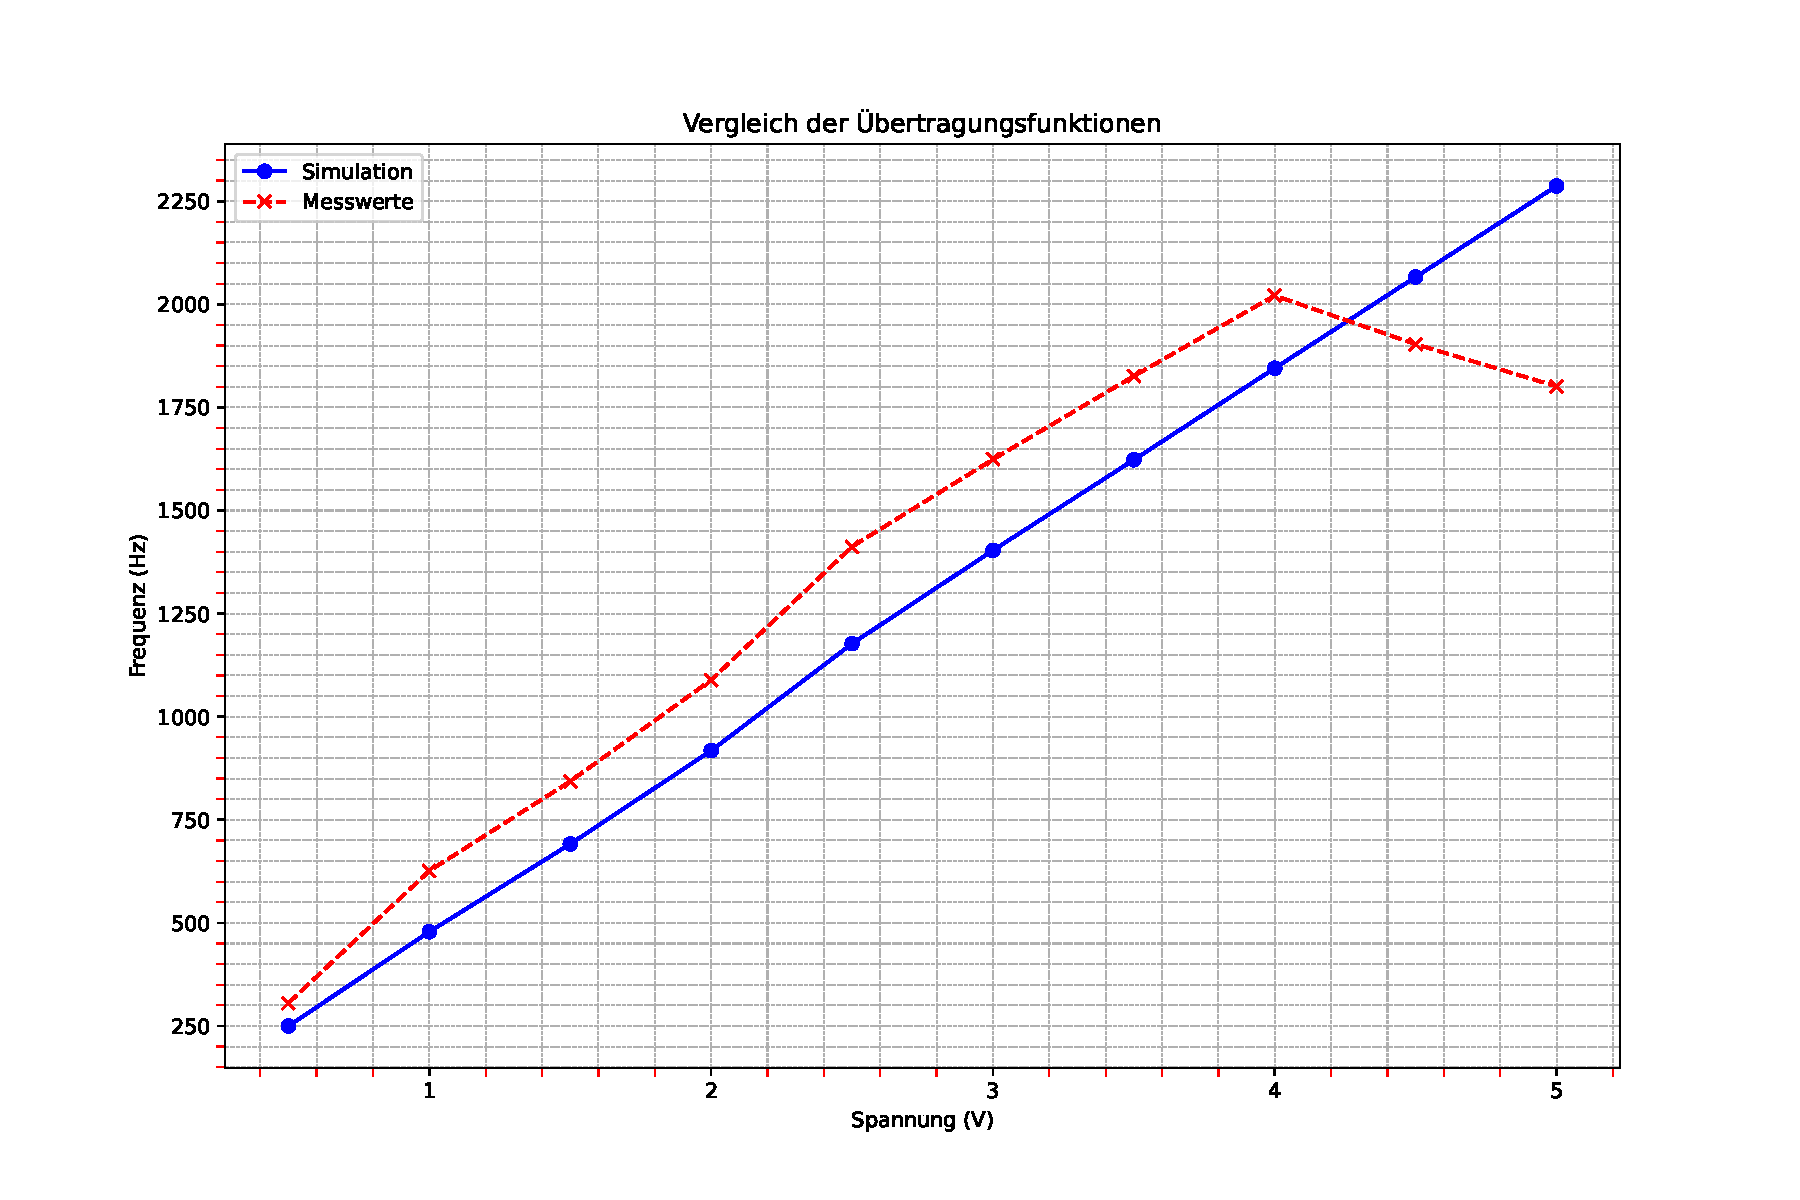
\includegraphics[width=1\linewidth]{Elektronik-Laborprotokoll_PLL/Abbildungen/frequenz_vergleich.pdf}
  \caption{VCO-Kennlinie}
  \label{fig:VCO_Kennlinie_Vergleich}
\end{figure}

Dargestellt ist die Ausgangsfrequenz in Abhängigkeit der Steuerspannung. Nach der Simulation steigt die Ausgangsfrequenz des Ausgangssignals proportional zur Steuerspannung. Im Idealfall sollte es eine Ausgangsfrequenz von \SI{2}{\kilo\hertz} bei einer Spannung von \SI{5}{\volt} zu erkennen sein, jedoch beträgt die Ausgangsfrequenz ungefähr \SI{2,3}{\kilo\hertz} auch bei der Simulation. Der Grund dafür ist, dass bei der Simulation auch nicht die idealen Werte für die Bauteile verwendet wurden. Es wurden die Bauteilwerten aus den E12-Reihe, was tatsächlich im Labor zu verwenden war, verwendet, damit nur die Abweichungen wegen der Messfehlern bzw. realen Bauteile zu beobachten sein können.

Im Ideallfall wäre bei \SI{5}{\volt} der Sollwert von \SI{2}{\kilo\hertz} zu erreichen. Dadurch würde das Verhältnis der Ausgangsfrequenz zur Spannung bzw. das Übertragungsfunktion beträgt nach der Simulation  $400\, \si{\hertz\per\volt}$ betragen. Jedoch ist die Übertragungsfunktion nach der Simulation beträgt genau wie bei den Messwerten ungefähr $450\, \si{\hertz\per\volt}$. Als Unterschied der Messwerten von der Simulation ist ein ungefähr konstant bleibender Offset im Intervall von \SI{0}{\volt} bis \SI{4}{\volt} zu beobachten, was auf die Eigenschaften der realen Bauteile zurückzuführen ist. Der Abfall bei der Ausgangsfrequenz trotz steigender Werte der Spannung im Intervall von \SI{4}{\volt} bis \SI{5}{\volt} bei den Messwerten lässt sich nicht mit den Eigenschaften realer Bauteile erklären. Es geht wahrscheinlich um einen großen Messfehler, dessen Grund nicht einfach zu erkennen ist. 

Mithilfe der linearen Regression lässt sich numerisch den Wert der konstanten Übertragungsfunktion $H_{VCO}$ nach der Messungen ermitteln. $H_{VCO}$ beträgt ungefähr $450\, \si{\hertz\per\volt}$, was im Laufe des Versuchs für die Dimensionierung weiterer Bauteile verwendet werden.





\subsection{Phasendetektor}

In der Phasenregelschleife dient der Phasendetektor dazu, die Phasendifferenz des VCOs und des Referenzsignals zu ermitteln. Der aufgebaute Phasendetektor bestimmt die Phasenabweichung in Form einer ternären Pulsweitenmodulation. Der aufzubauende Phasendetektor reagiert auf die steigende Flanken der Eingangssignale. Das obere D-Flipflop wird durch die steigende Flanke eines Signals gesetzt, und das untere Flipflop wird durch die steigende Flanke des anderen Signals gesetzt.

 Wenn beide Flipflops auf High sind, werden beide durch das AND-Gatter in der Rückkopplung zurückgesetzt. Abhängig davon, welches Flipflop gerade gesetzt ist, gibt der nachfolgende Subtrahierer eine positive oder negative Spannung aus.
Je hochfrequenter das Referenzsignal als das vom VCO erzeugte Signal, desto häufiger ist das Ausgangssignal des Subtrahierers positiv, je niederfrequenter das Referenzsignal als das vom VCO erzeugte Signal, desto häufiger ist das Ausgangssignal des Subtrahierers negativ. Durch den integrativen Anteil des Schleifenfilters wird so eine
Steuerspannung für den VCO erzeugt, die je nach Phasenversatz und Frequenzdifferenz nach unten oder oben korrigiert wird. \cite{Skript}

\begin{figure}[H]
  \centering
  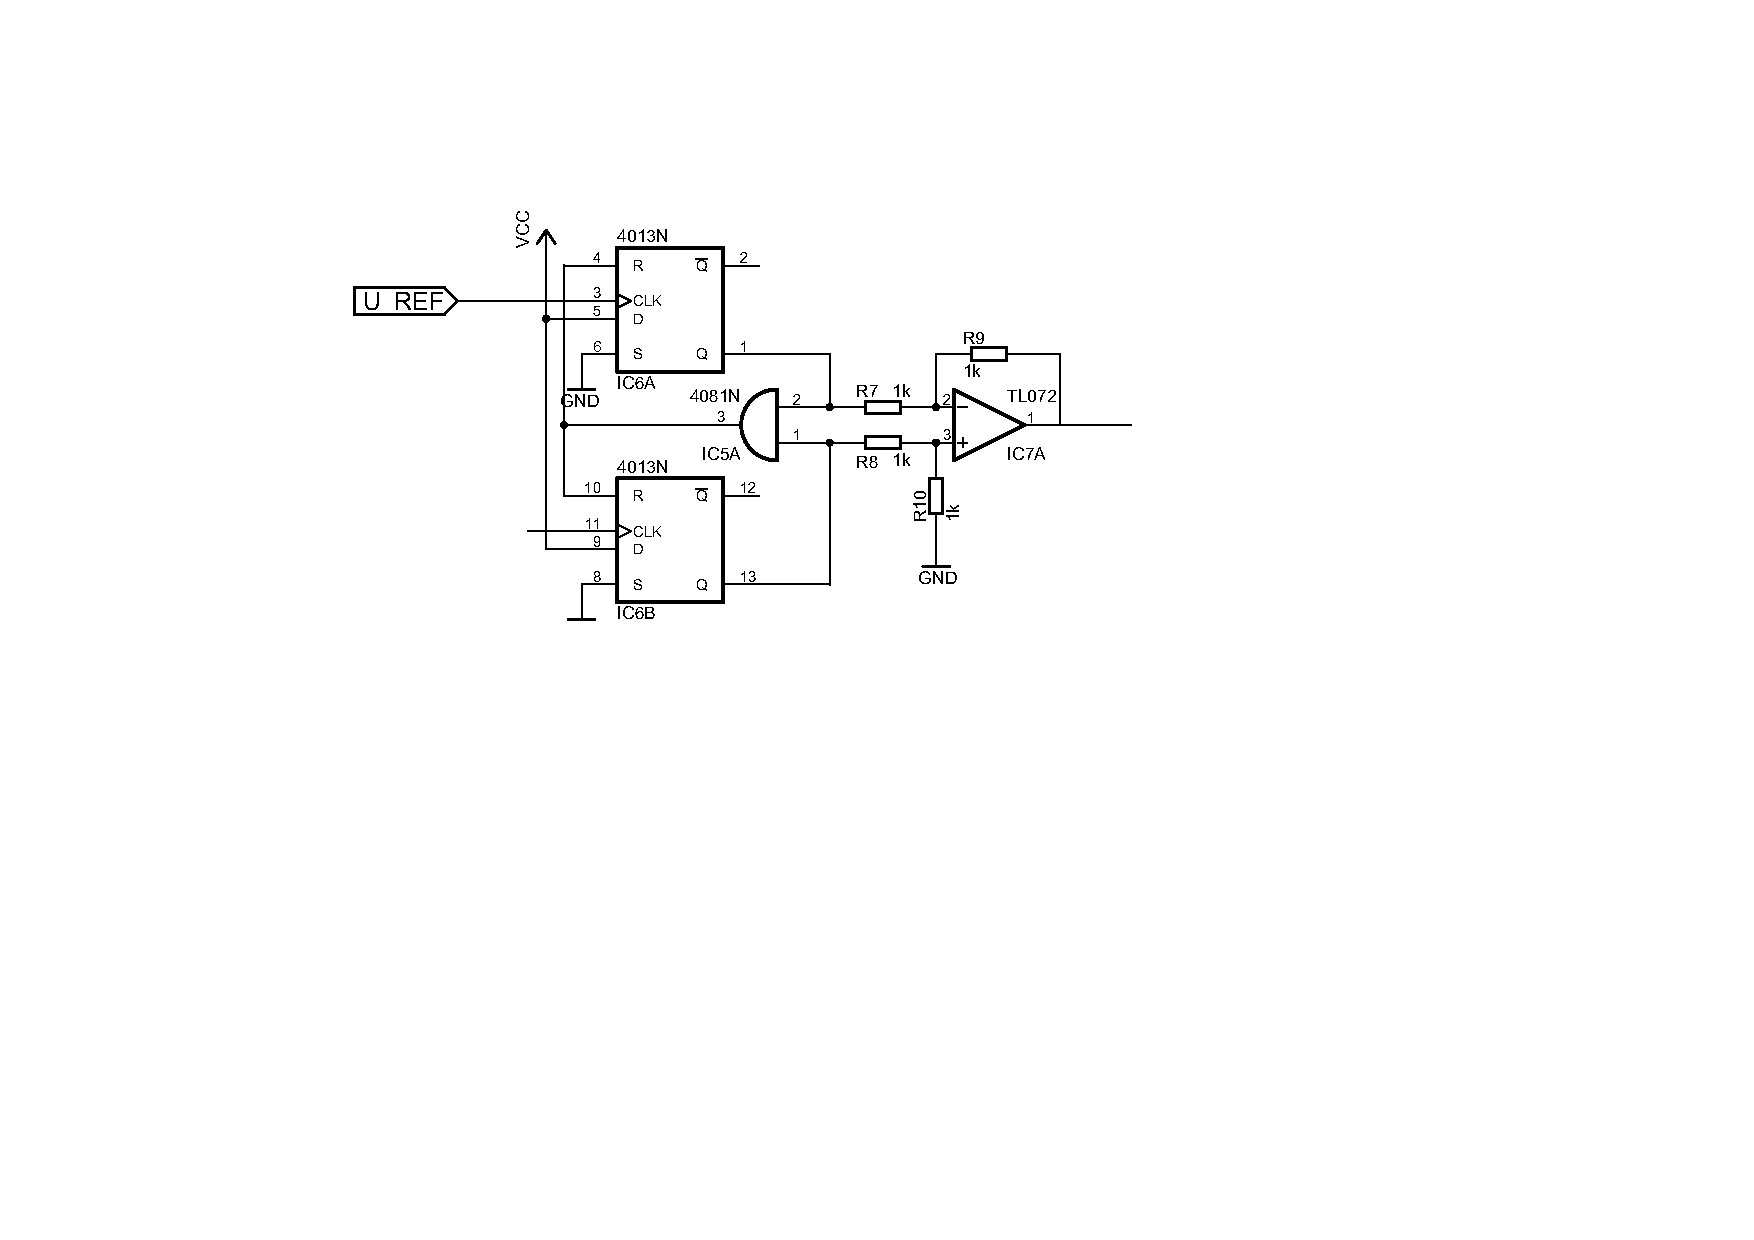
\includegraphics[width=0.8\linewidth]{Elektronik-Laborprotokoll_PLL/Abbildungen/Phasendetektor_Schaltung.pdf}
  \caption{Phasendetektor (Schaltplan)}
  \label{fig:PD_Schaltung}
\end{figure}

In den Abbildungen \ref{fig:kleiner_als_1k} und \ref{fig:mehr_als_1k} befinden sich zwei Fälle als Beispiel dafür, wie der Phasendetektor auf den Phasenunterschied zweier Referenzsignale reagiert.

\begin{figure}[H]
  \centering
  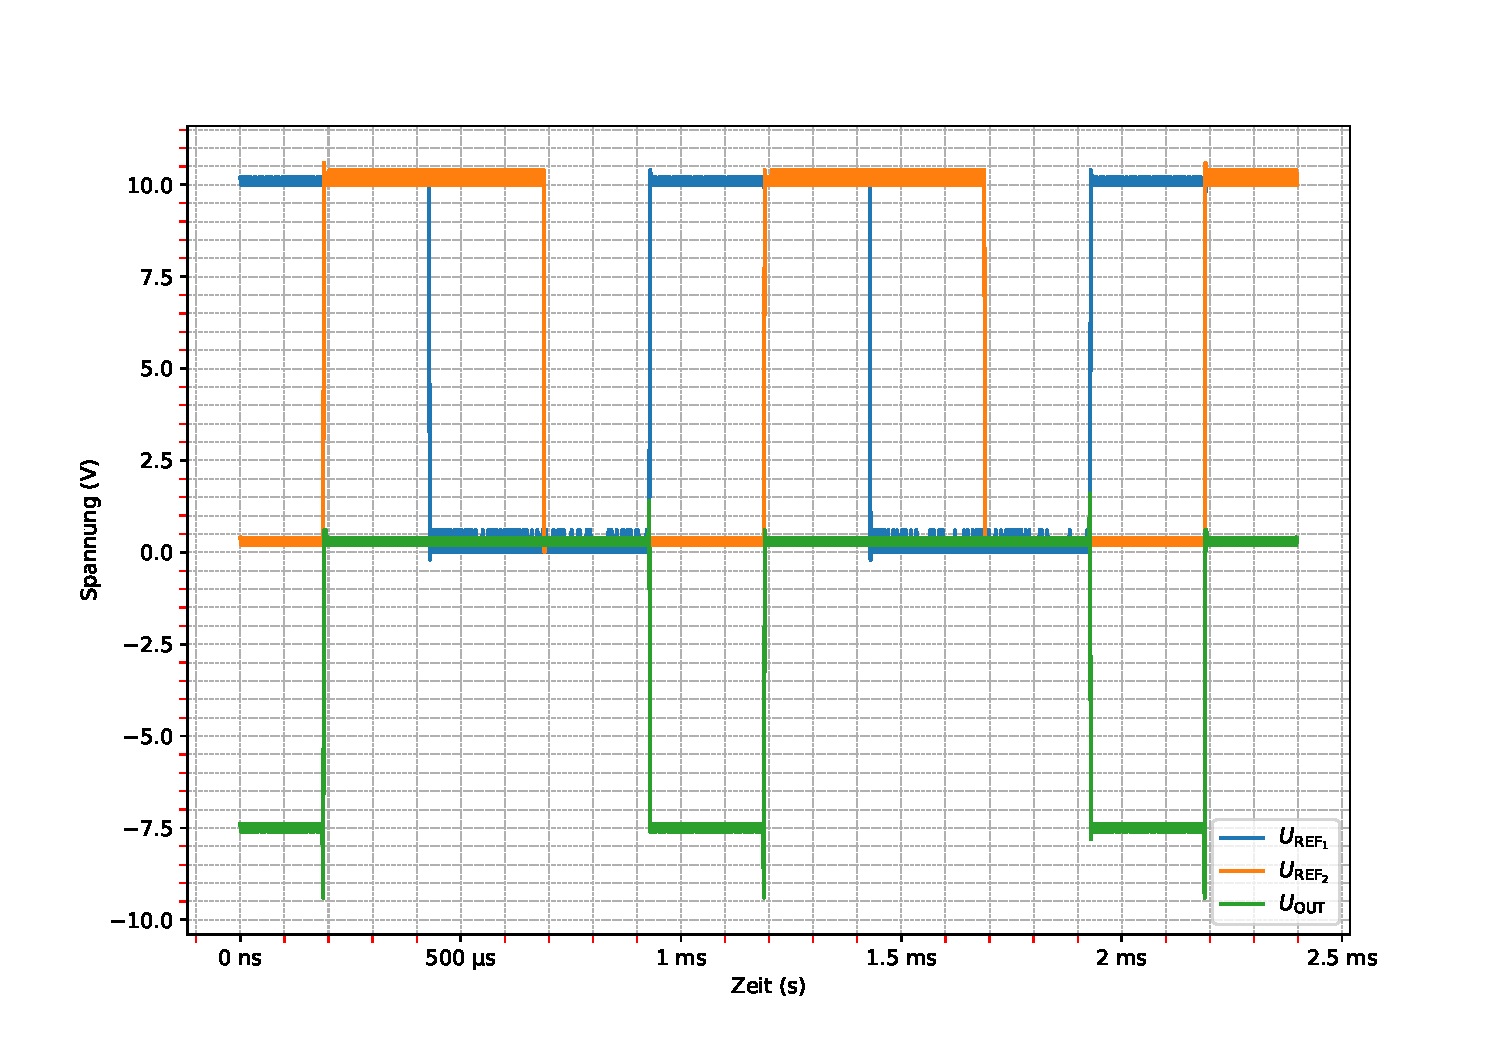
\includegraphics[width=0.8\linewidth]{Elektronik-Laborprotokoll_PLL/Plots/klein_als_1k_unten.pdf}
  \caption{Phasendetektor, Beispiel 1}
  \label{fig:kleiner_als_1k}
\end{figure}

Die Abbildung \ref{fig:kleiner_als_1k} stellt das erste Beispiel für die Funktionsweise des Phasendetektors dar. Die Signale am Eingang des Phasendetektors sind beide Rechtecksignale mit einer Amplitude von \SI{10}{\volt}. Das Eingangssignal 2 eilt in diesem Beispiel vor. Der Phasendetektor reagiert auf die steigende Flanken beider Eingangssignale. Bei $t=\SI{0}{\nano\second}$ befindet sich das Ausgangssignal bei seinem minimalen Wert bei ungefähr \SI{-7,5}{\volt}. Dann reagiert er auf die steigende Flanke des Eingangssignals 2, sodass das Ausgangssignal auf eine Spannung von \SI{0}{\volt} steigt. Das Ausgangssignal bleibt bei \SI{0}{\volt} konstant, bis das Eingangssignal 1 eine steigende Flanke hat. Bei ungefähr \SI{0,9}{\milli\second} hat das Eingangssignal 1 eine steigende Flanke, so dass das Ausgangssignal zurück zu seinem minimalen Wert bzw. auf \SI{-7,5}{\volt} sinkt. Warum es nicht auf \SI{-10}{\volt} sinkt, liegt es an nicht idealen Eigenschaften der verwendeten Bauteile. Der Ausgangssignal bleibt bei diesem Wert, bis das Eingangssignal 2 eine neue steigende Flanke besitzt. Dieses Verhalten des Ausgangssignals wiederholt sich periodisch. Zusammengefasst hat das Ausgangssignal eine steigende Flanke, wenn das Eingangssignal 2 eine steigende Flanke hat, und es hat eine fallende Flanke, wenn das Eingangssignal 1 eine steigende Flanke hat.

\begin{figure}[H]
  \centering
  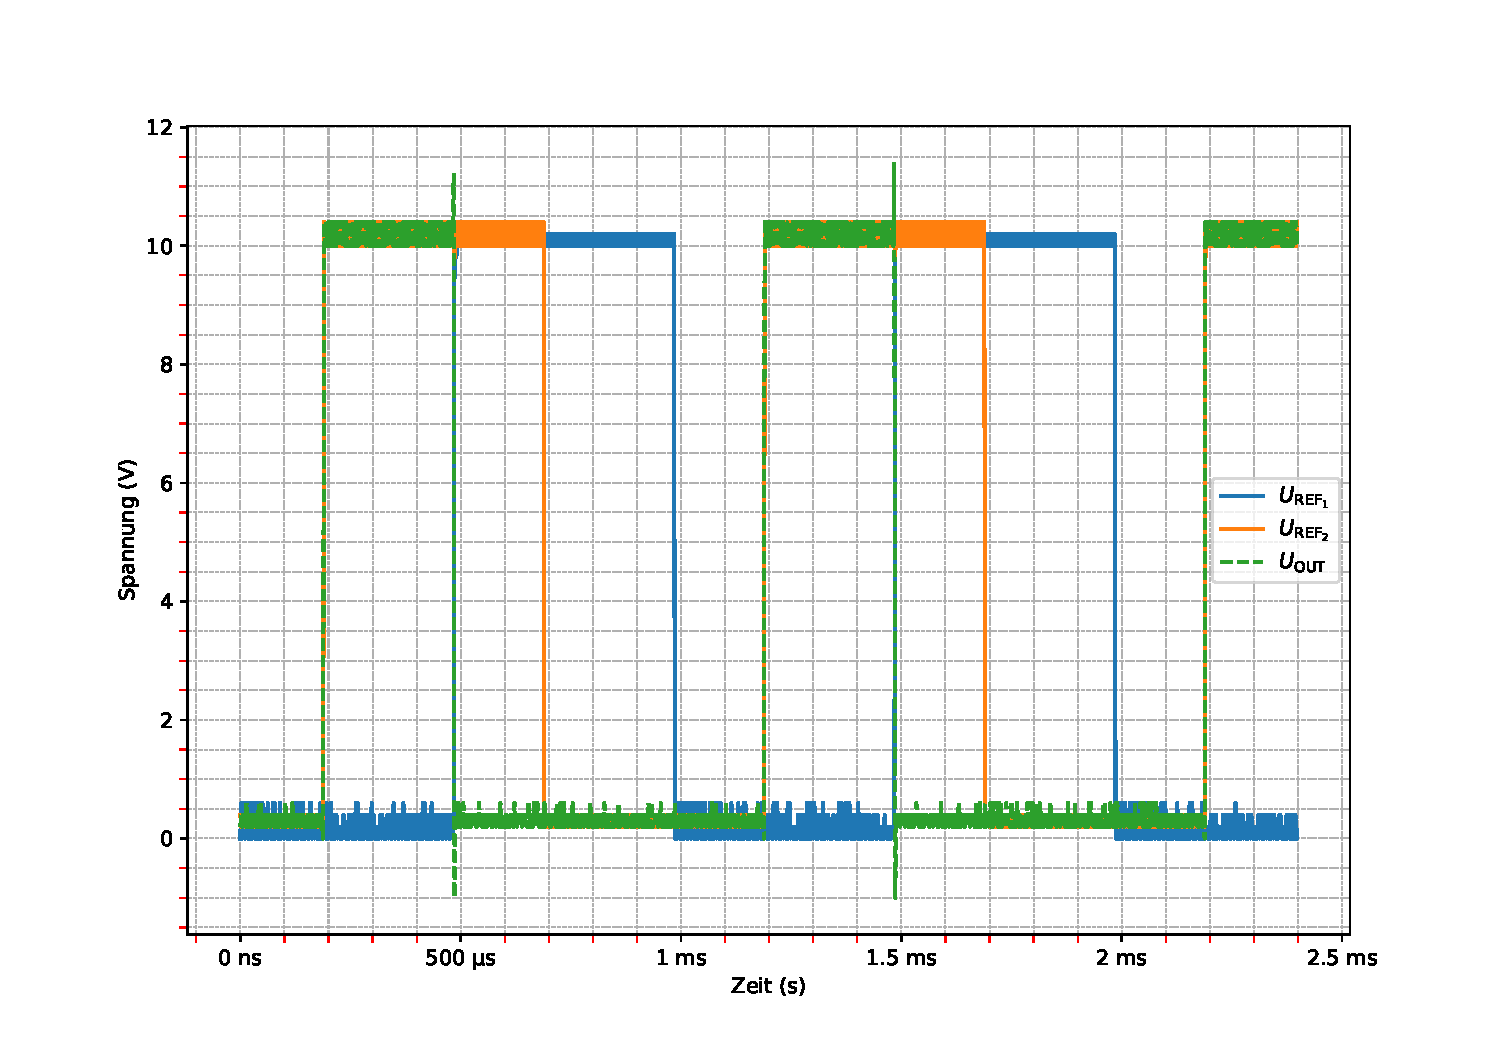
\includegraphics[width=0.8\linewidth]{Elektronik-Laborprotokoll_PLL/Plots/mehr_als_1k_oben-1.pdf}
  \caption{Phasendetektor, Beispiel 2}
  \label{fig:mehr_als_1k}
\end{figure}

Die Abbildung \ref{fig:mehr_als_1k} stellt ein zweites Beispiel für die Funktionsweise des Phasendetektors dar. In diesem Beispiel eilt das Einganssignal $U_1$ vor. Wie im ersten Beispiel reagiert sich der Phasendetektor auf die steigende Flanken der Eingangssignale. Wenn das Eingangssignal $U_1$ eine steigende Flanke hat, hat das Ausgangssignal eine steigende Flanke und wenn das Eingangssignal $U_2$ eine steigende Flanke hat, hat das Ausgangssignal eine fallende Flanke. Im Gegensatz zum ersten Beispiel schwingen die Werte des Ausgangssignals in positiven Werten bzw. zwischen \SI{0}{\volt} und \SI{10}{\volt}. 

Das Übertragungsverhalten,was eine Konstante ist, eines Phasendetektors kann beschrieben werden als das Verhältnis zwischen dem Ausgangsspannungsbereich und dem Arbeitsbereich des Phasendetektors. 

Die Abbildung \ref{fig:4pi} zeigt den Arbeitsbereich des Phasendetektors.
\begin{figure}[H]
  \centering
  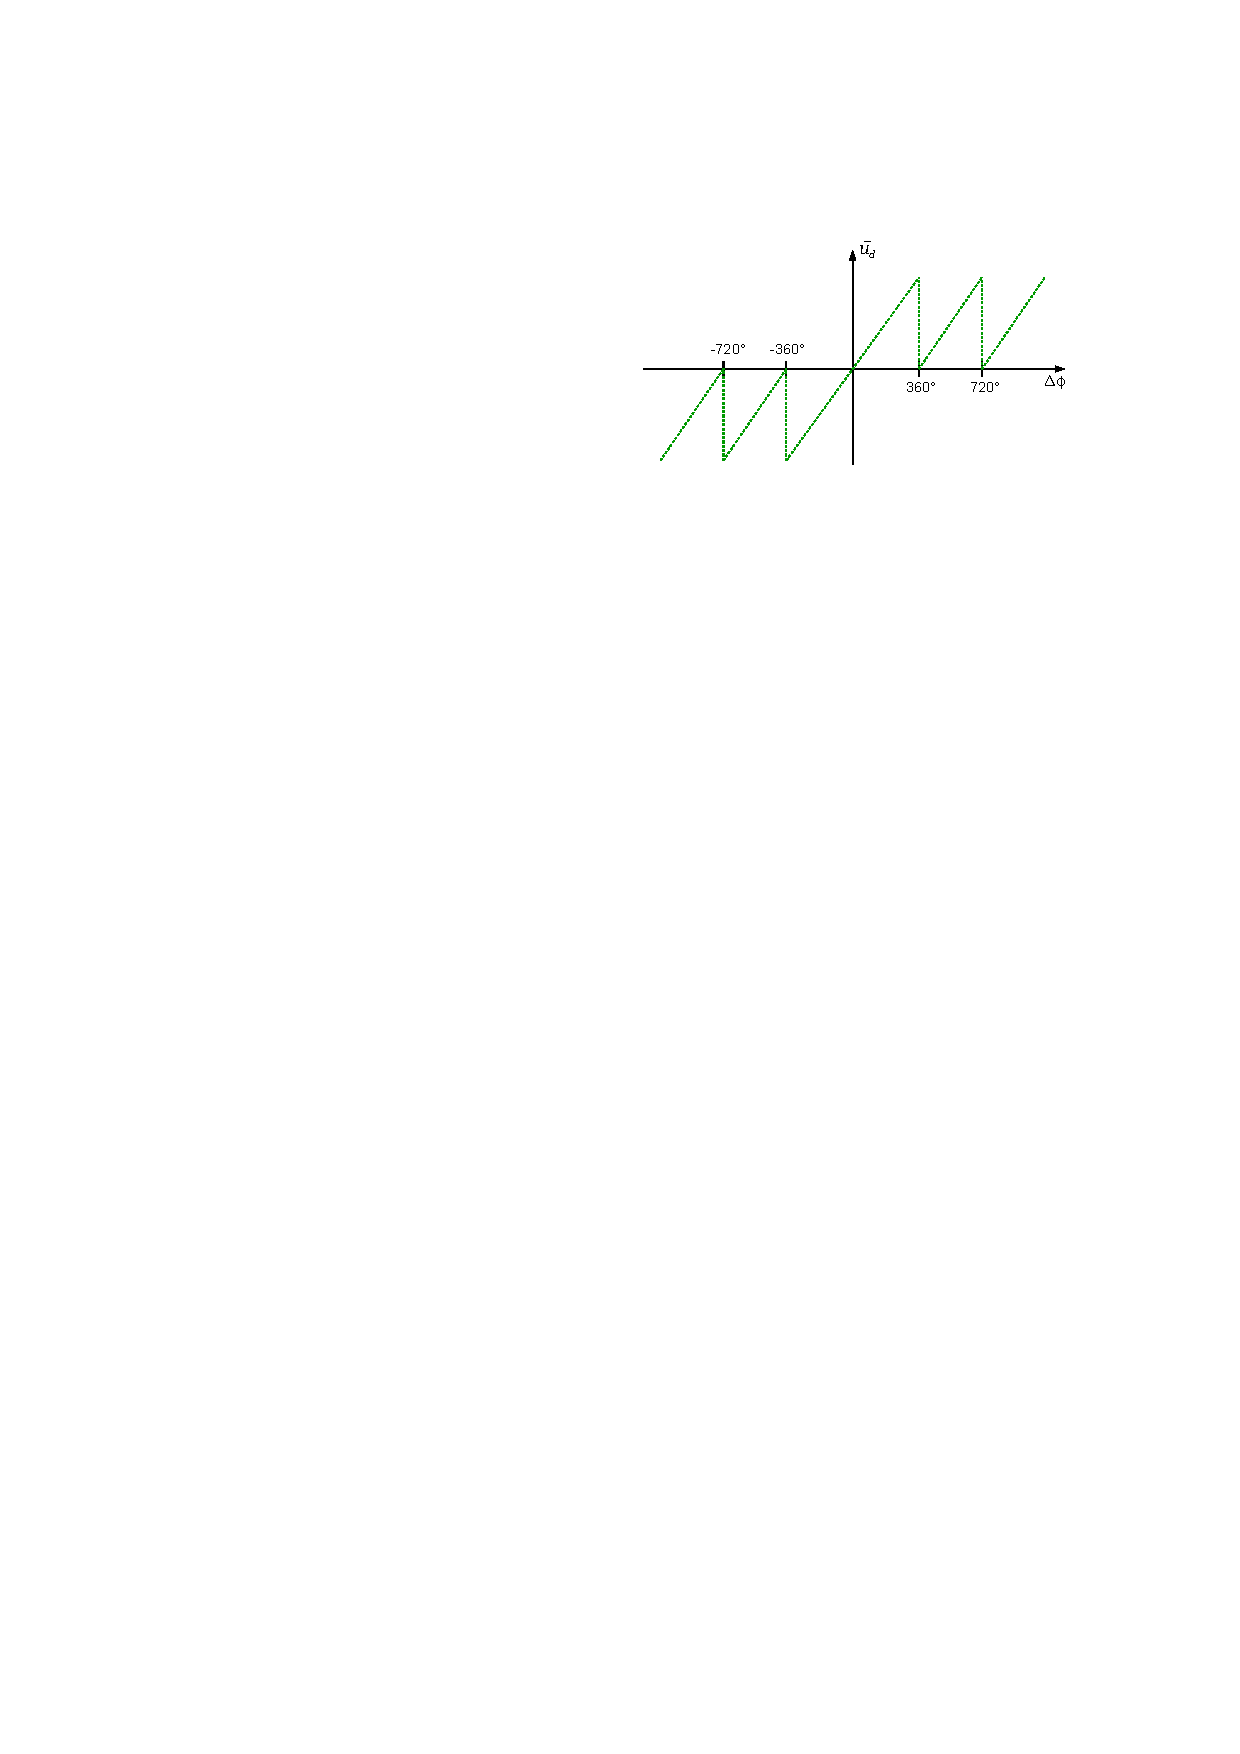
\includegraphics[width=0.8\linewidth]{Elektronik-Laborprotokoll_PLL/Abbildungen/Geheimnis_4pi.pdf}
  \caption{Arbeitsbereich des Phasendetektors \cite{Skript}}
  \label{fig:4pi}
\end{figure}

\begin{equation}
H_{\text{PD}} = \frac{\Delta U_{\text{aus}}}{\Delta \varphi_{\text{max}}} = \frac{U_{\text{aus,max}} - U_{\text{aus,min}}}{\Delta \varphi_{\text{max}}}
\end{equation}

Durch die Einsetzung der gemessenen Werte in die Gleichung folgt:
\begin{align*}
H_{\text{PD}}=\frac{\SI{10,4}{\volt}-(\SI{-8,3}{\volt})}{4\pi}\approx \SI{1,49}{\volt}
\end{align*}





\subsection{Schleifenfilter}

Als Schleifenfilter wird ein PI-Filter aufgebaut.

\begin{figure}[H]
  \centering
  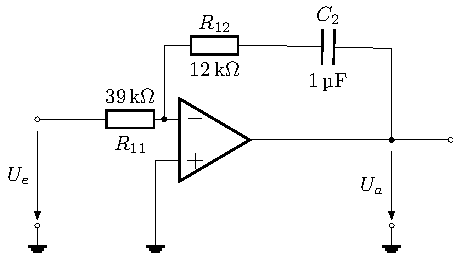
\includegraphics[width=0.4\linewidth]{Elektronik-Laborprotokoll_PLL/Abbildungen/Schleifenfilter_Schaltung.pdf}
  \caption{PI-Filter (Schaltplan)}
  \label{fig:PI-Filter_Schaltung}
\end{figure}

Die PI-Filter hat die folgende Übertragungsfunktion  \cite{SkriptElektronik}:

\begin{equation}
H(s)_{\text{PI}} = \frac{s \cdot R_2 C_2 + 1}{s \cdot R_1 C_2}
\end{equation}

Es wird so abgekürzt: $\tau_i=R_i C_2$ für $i\in\{1,2\}$

Die Übertragungsfunktion des geschlossene Regelkreises(PLL) lautet nach dem Blockschaltbild \cite{Skript} wie folgt:

\begin{equation}
H_{PLL} = \frac{\varphi_{VCO}}{\varphi_{\text{ref}}} = \frac{H_{PD}(s) H_{LP}(s)H_{VCO}(s)}{s +H_{PD}(s)  H_{LP}(s)H_{VCO}(s)}
\end{equation}

Die Übertragungsfunktion des Phasendetektors und der VCO sind als Konstante betrachtet werden, somit folgt:
\begin{equation}
\label{eq:PLL_1}
H_{PLL} = \frac{H_{PD}H_{VCO}H_{LP}(s)}{s +H_{PD}  H_{LP}(s)H_{VCO}}
\end{equation}

Das Verhalten der PLL wird hauptsächlich durch das Schleifenfilter beeinflusst. Die Übertragungsfunktion der PLL lässt sich auch folgendermaßen beschreiben \cite{SkriptElektronik}:

\begin{equation}
\label{eq:PLL_2}
H_{PLL} = \frac{2s\delta\omega_n+\omega^2_n}{s^2+2s\omega_n+\omega^2_n}
\end{equation}

Durch die Gleichsetzung der Gleichungen \ref{eq:PLL_1} und \ref{eq:PLL_2} lassen sich die Gleichungen der $\omega_n$ als natürliche Frequenz und $\delta$ als Dämpfung bestimmen.

\begin{align}
 H_{PLL} = \frac{H_{PD}H_{VCO}H_{LP}(s)}{s +H_{PD}  H_{LP}(s)H_{VCO}}= \frac{2s\delta\omega_n+\omega^2_n}{s^2+2s\omega_n+\omega^2_n}  
\end{align}

Für $H_{LP}(s)$ wird die Übertragungsfunktion der PI-Filter wird eingesetzt:
\begin{align*}
 H_{PLL} = \frac{H_{PD}H_{VCO}\cdot \frac{s \cdot \tau_2 + 1}{s \cdot \tau_1}}{s +H_{PD} H_{VCO}\cdot \frac{s \cdot \tau_2 + 1}{s \cdot \tau_1}}= \frac{2s\delta\omega_n+\omega^2_n}{s^2+2s\omega_n+\omega^2_n}  
\end{align*}
\begin{align*}
 H_{PLL} = \frac{\frac{H_{PD}H_{VCO}\cdot (s \cdot \tau_2 + 1)}{{s \cdot \tau_1}}}{\frac{s^2\tau_1 +H_{PD} H_{VCO}\cdot (s \cdot \tau_2 + 1)}{{s \cdot \tau_1}}}= \frac{2s\delta\omega_n+\omega^2_n}{s^2+2s\omega_n+\omega^2_n}  
\end{align*}

\begin{align*}
 H_{PLL} = \frac{H_{PD}H_{VCO}\cdot (s \cdot \tau_2 + 1)}{s^2\tau_1 +H_{PD}H_{VCO}\cdot (s \cdot \tau_2 + 1)}= \frac{2s\delta\omega_n+\omega^2_n}{s^2+2s\omega_n+\omega^2_n}  
\end{align*}

Durch die Umforumung folgt:
\begin{align*}
 H_{PLL} = \frac{s( H_{PD}\cdot H_{VCO}\cdot \tau_2)- H_{PD}\cdot H_{VCO}}{s^2\tau_1+s\cdot(H_{PD}\cdot H_{VCO}\cdot \tau_2)+H_{PD}\cdot H_{VCO}}= \frac{2s\delta\omega_n+\omega^2_n}{s^2+2s\omega_n+\omega^2_n}  
\end{align*}

Durch einige Erweiterungen der Gleichung in der linken Seite folgt:
\begin{align*}
 H_{PLL} = \frac{2s\cdot(\frac{H_{PD}\cdot H_{VCO}\cdot \tau_2}{\tau_1 \cdot 2})+(\frac{H_{PD}\cdot H_{VCO}}{\tau_1})}{s^2+2s\cdot(\frac{H_{PD}\cdot H_{VCO}\cdot \tau_2}{\tau_1 \cdot 2})+(\frac{H_{PD}\cdot H_{VCO}}{\tau_1})} = \frac{2s\delta\omega_n+\omega^2_n}{s^2+2s\omega_n+\omega^2_n}  
\end{align*}

Durch den Koeffizientenvergleich folgen für $\omega_n$ und $\delta$ folgende Gleichungen:
\begin{equation}
\label{eq:omega}
\omega_{n,\text{PI}} = \sqrt{\frac{H_{\text{PD}} \cdot H_{\text{VCO}}}{\tau_1}}
\end{equation}
und
\begin{equation}
\label{eq:delta}
\delta_{PI}=\frac{\omega_{n,PI}\cdot \tau_2}{2}
\end{equation}

$\tau_1$ und $\tau_2$ wurden wie folgt definiert:

\begin{align}
\tau_1 &= R_{11} \cdot C_1 \\
\tau_2 &= R_{12} \cdot C_1
\end{align}



Durch die Umformung der Gleichung \ref{eq:omega} nach $\tau_1$ folgt:

\begin{align}
\label{align:tau1}
\tau_1=\frac{H_{\text{PD}}\cdot H_{\text{VCO}}}{\omega_{n,\text{PI}}^2}
\end{align}

Der gegebene Wert für $\omega_{n,\text{PI}}$ ist wie folgt:

\begin{equation}
\omega_{n,\text{PI}}=2\pi \cdot \SI{20}{\hertz}
\end{equation}


Durch die Einsetzung der berechneten Werte für $H_{PD}$ und $H_{VCO}$ und den gegebenen Wert für $\omega_{n,PI}$ in die Gleichung \ref{align:tau1} folgt:

\begin{align}
\tau_1 &= \frac{\SI{1.49}{\volt} \cdot 450\, \si{\hertz\per\volt}}{(2\pi \cdot \SI{20}{\hertz})^2}=\SI{0,042460}{\second}
\end{align}



Ausgewählt ist ein Kondensator mit einer Kapazität von $C_1$=\SI{1}{\micro\farad}.Aus der Gleichung $\tau_1= R_{11} \cdot C_1$ lässt sich $R_{11}$ bestimmen:

\begin{align}
R_{11}=\frac{\tau_1}{C_1}=\frac{\SI{0,042460}{\second}}{\SI{1}{\micro\farad}}=\SI{42460}{\ohm}
\end{align}

Als nächster Wert für den berechneten Widerstand wird ein Wert aus der E12-Widerstandsreihe ausgewählt, sodass $R_{11}$=\SI{39}{\kilo\ohm} beträgt. 

Durch die Umformung der Gleichung \ref{eq:delta} nach $\tau_2$ folgt:

\begin{equation}
\tau_2= \frac{ 2 \cdot \delta_{PI}}{\omega_{n,PI}}
\end{equation}


Nach dem Filtermodell von Butterworth beträgt $\delta \approx 0,7$.

Wenn man die gegebenen Werte in die Gleichung einsetzt, lässt sich $\tau_2$ bestimmen:
\begin{equation}
\tau_2= \frac{ 2 \cdot 0,7}{2\pi \cdot \SI{20}{\hertz}}=\SI{0,011141}{\second}
\end{equation}

Ausgewählt war ein Kondensator mit einer Kapazität von $C_1$=\SI{1}{\micro\farad}.Aus der Gleichung $\tau_2= R_{12} \cdot C_1$ lässt sich $R_{12}$ bestimmen:

\begin{align}
R_{12}=\frac{\tau_2}{C_1}=\frac{\SI{0,011141}{\second}}{\SI{1}{\micro\farad}}\approx \SI{11141}{\ohm}
\end{align}

Als nächster Wert für den berechneten Widerstand wird ein Wert aus der E12-Widerstandsreihe ausgewählt, sodass $R_{12}$=\SI{12}{\kilo\ohm} beträgt.


Die Abbildung \ref{fig:Bode} zeigt das Bodediagramm des aufgebauten PI-Filter verglichen mit den Simulationswerten.

\begin{figure}[H]
  \centering
  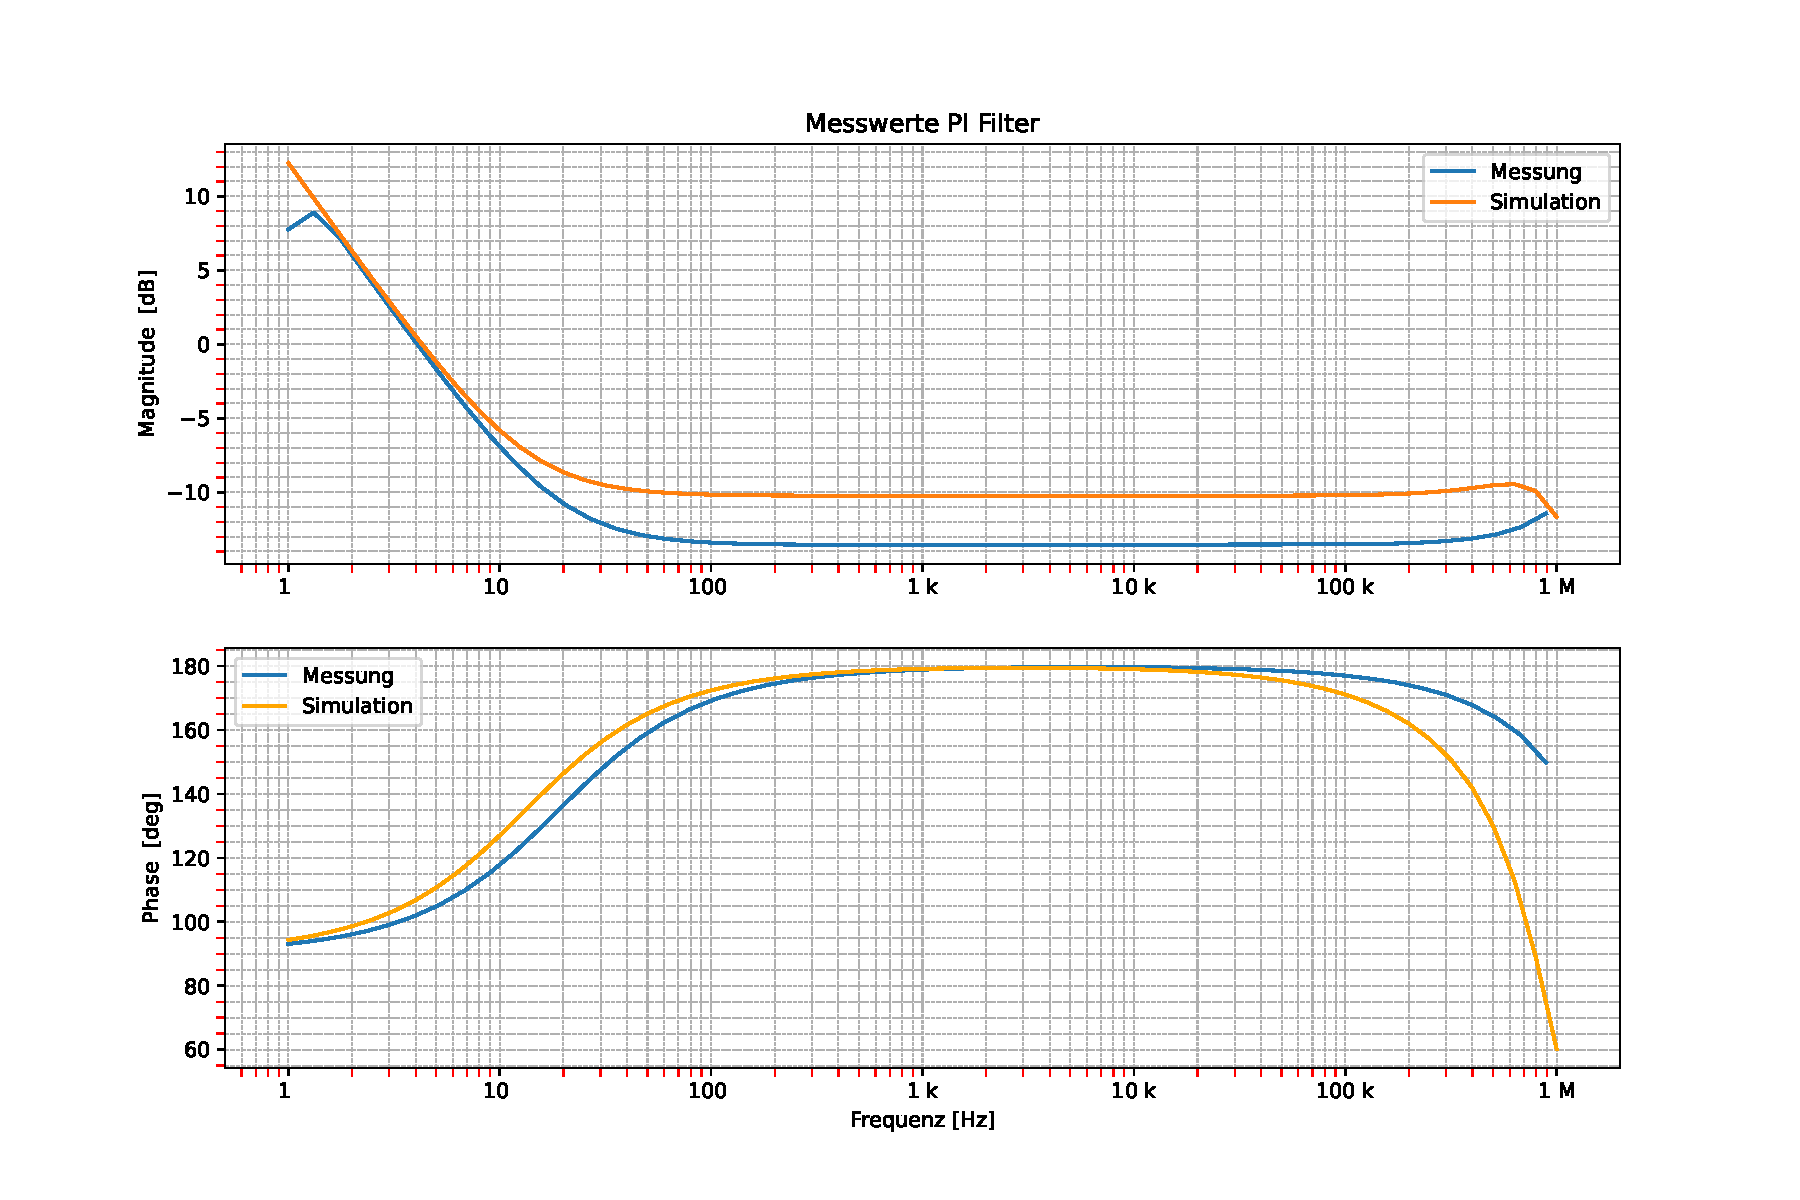
\includegraphics[width=0.8\linewidth]{Elektronik-Laborprotokoll_PLL/Abbildungen/PI_Filter_Bode.pdf}
  \caption{PI-Filter-Bodediagramm}
  \label{fig:Bode}
\end{figure}

Bei dem PI Filter ist die Amplitudenverstärkung für tiefere Frequenzen größer. Wenn sich die Frequenz des Eingangssignals an die \SI{0}{\hertz} nähert, läuft die Verstärkung des PI-Filters wegen des I-Anteils gegen unendlich. Die Verstärkung des Integrators verringert sich um mit höheren Frequenze.  Wenn sich die Frequenz des Eingangssignals an die $\infty$ nähert, läuft die Verstärkung des PI-Filters gegen \SI{0}{\decibel}, bzw. 1.\\
Die Messwerte stimmmen für Frequenzen bis \SI{100}{\kilo\hertz} gut mit der Simulation überein. Die deutliche Abweichung, was nicht mit der externen Schaltung erklärt werden kann, bei höheren Frequenzen als \SI{100}{\kilo\hertz} ist in die Charakteristik des verwendeten OPVs zurückzuführen.\\
%\subsubsection{Korrektur:}




\subsection{Die PLL als integrierte Schaltungseinheit}

Der VCO, der Phasendetektor und das Schleifenfilter bilden zusammen die Phasenregelschleife, wie in Abbildung \ref{fig:PLL_KiCad} dargestellt ist.

\begin{figure}[H]
  \centering
  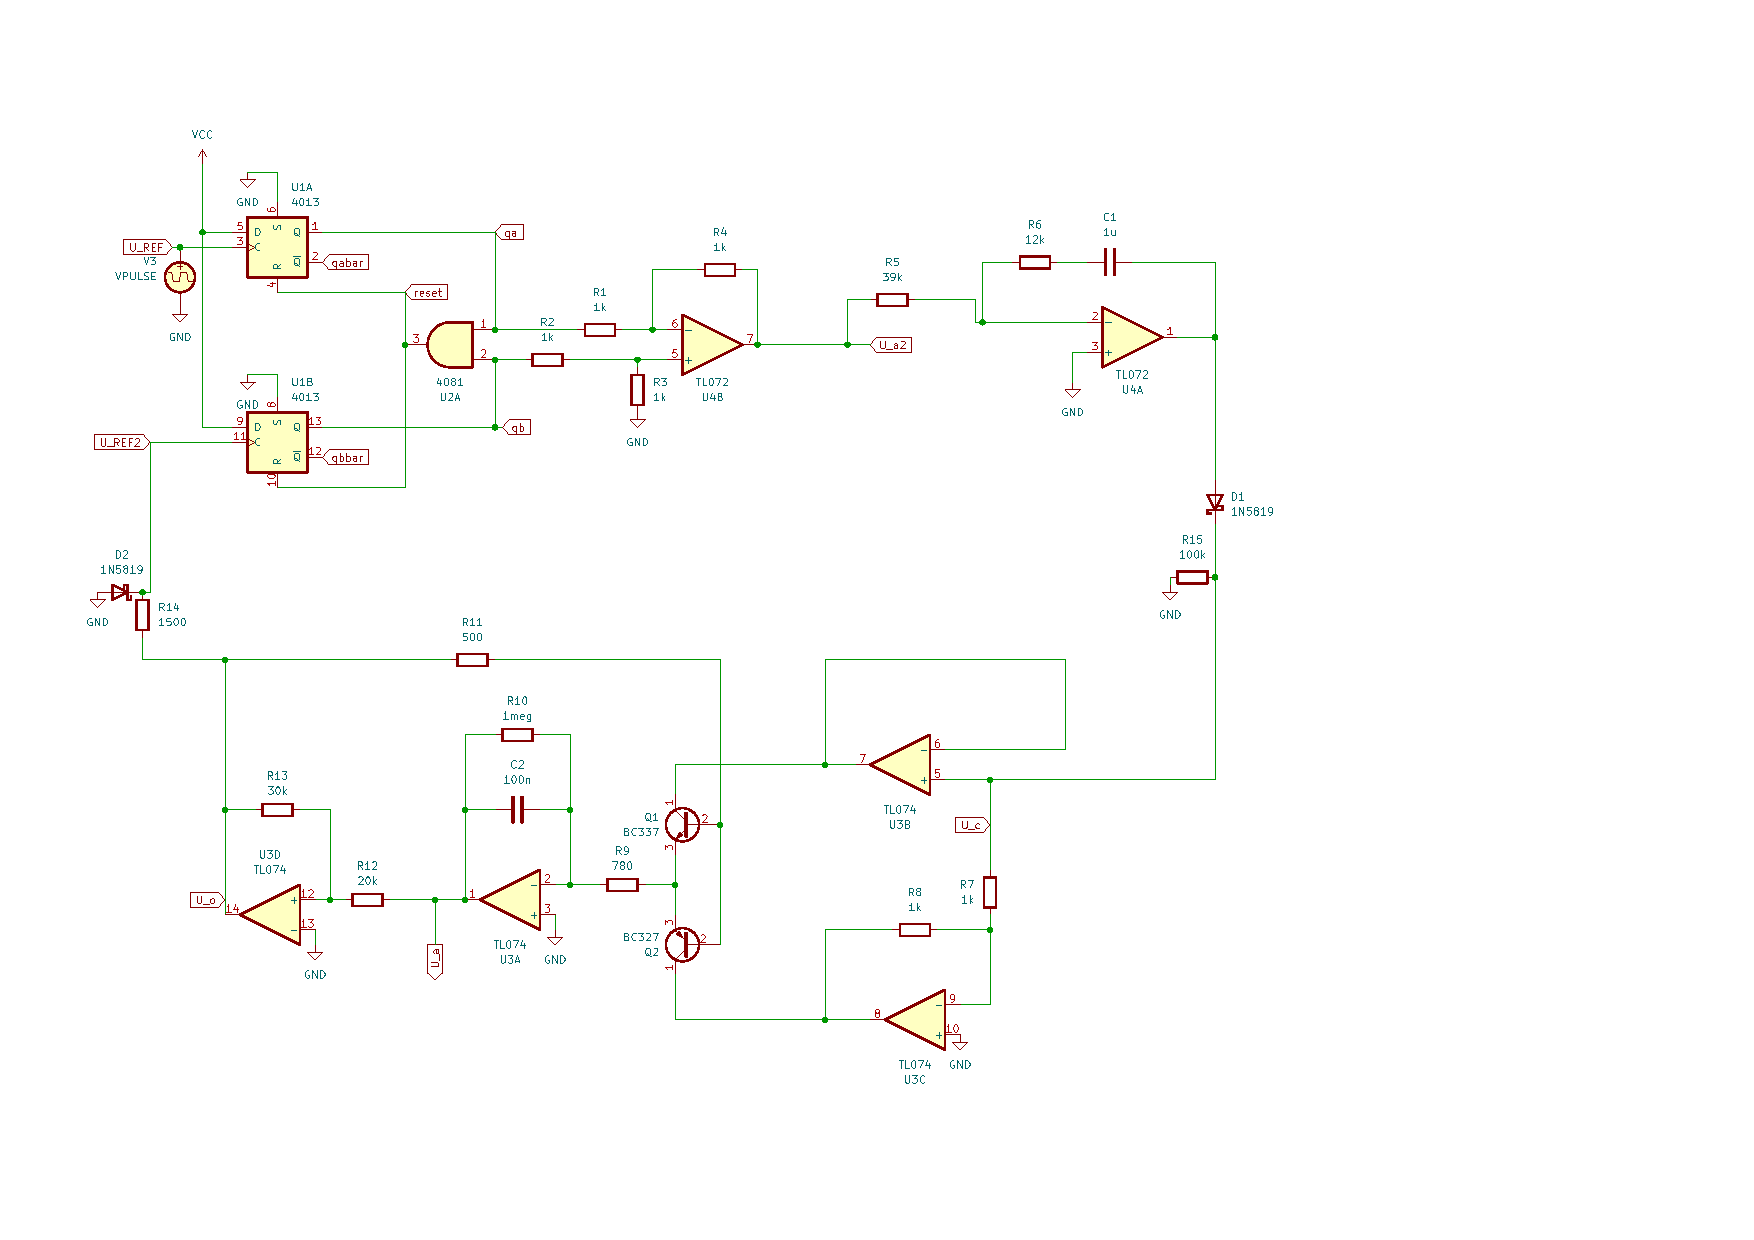
\includegraphics[width=0.8\linewidth]{Elektronik-Laborprotokoll_PLL/Abbildungen/PLL_KiCad.pdf}
  \caption{Zusammenbau der PLL}
  \label{fig:PLL_KiCad}
\end{figure}

Die Abbildung \ref{fig:spa_ges} zeigt das Oszilloskopbild für die gesamte Schaltung der PLL.

\begin{figure}[H]
  \centering
  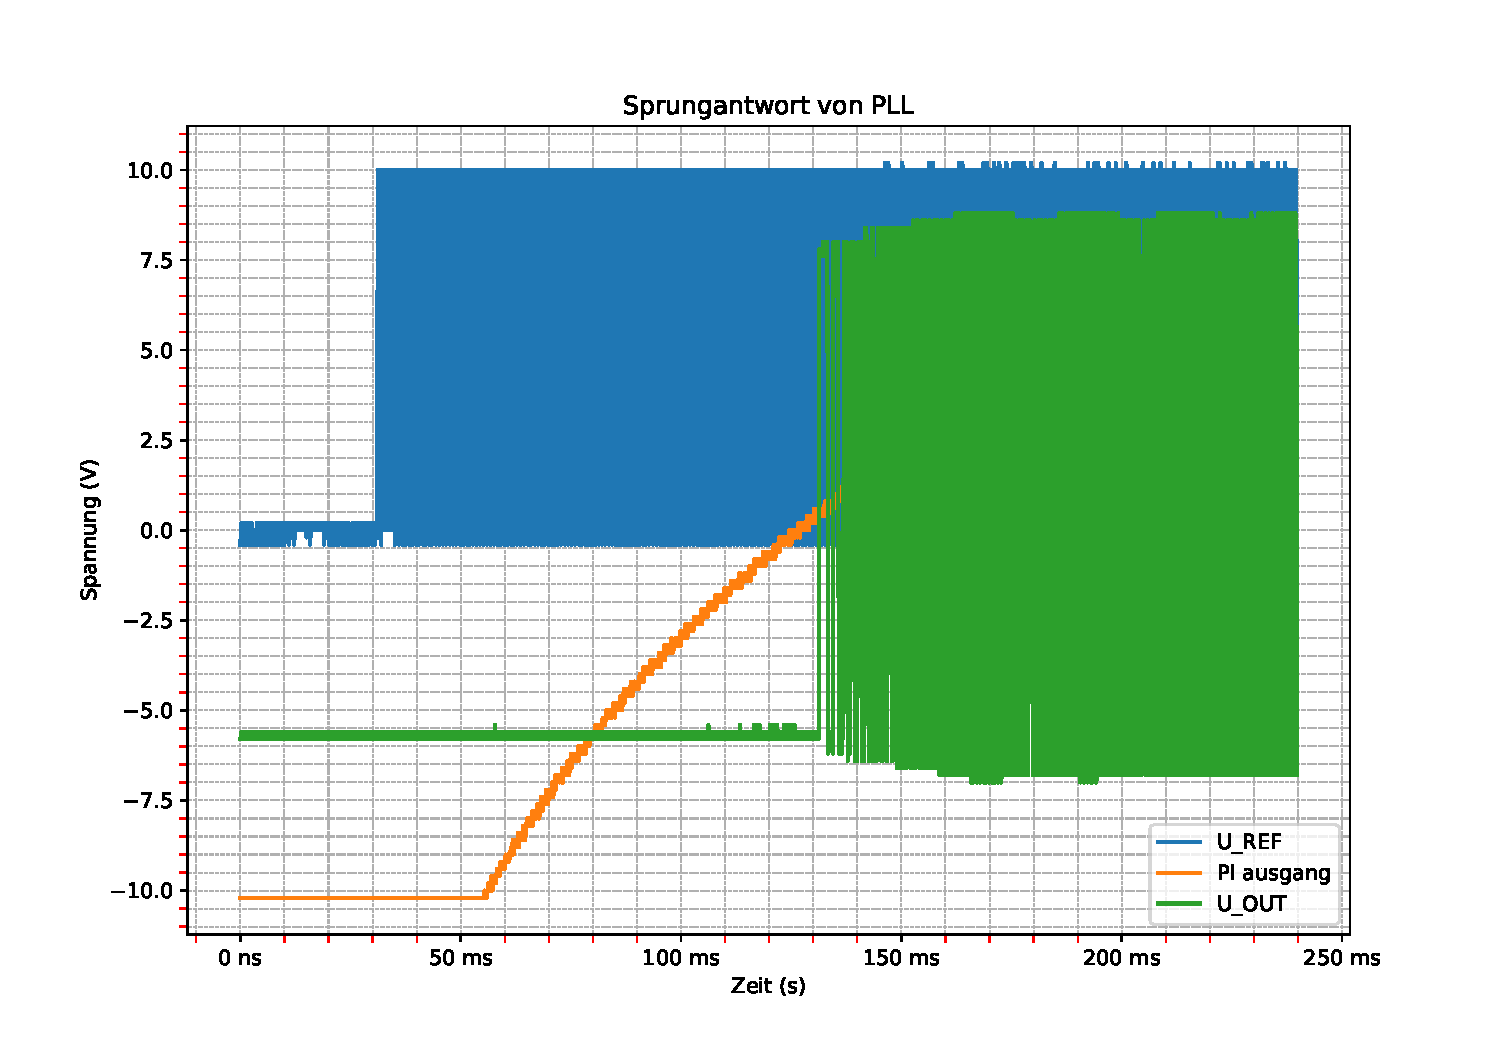
\includegraphics[width=1\linewidth]{Elektronik-Laborprotokoll_PLL/Abbildungen/sprungantwort_gesamt.pdf}
  \caption{Dynamisches Verhalten des PLL-Systems mit PI-Filter im Zeitbereich}
  \label{fig:spa_ges}
\end{figure}

Im dargestellten Diagramm wird das dynamische Verhalten eines Phasenregelschleifen-Systems (PLL) mit einem PI-Filter als Schleifenfilter im Zeitbereich visualisiert. Zu Beginn befindet sich das Referenzsignal $U_{\text{REF}}$ bei 0V, während der PI-Ausgang bei -12V und $U_{\text{OUT}}$ bei -6V startet. Durch eine induzierte Oszillation im $U_{\text{REF}}$ reagieren der Phasenkomparator und das PI-Filter mit einer Spannungserhöhung. Zunächst erreicht $U_{\text{OUT}}$ jedoch nicht die Schwelle für die Oszillation, wodurch eine Verzögerung entsteht. Nach einigen Millisekunden beginnt $U_{\text{OUT}}$ zwischen 7V und -7V zu oszillieren. Beide, $U_{\text{REF}}$ und $U_{\text{OUT}}$, oszillieren nun, und der spannungsgesteuerte Oszillator (VCO) versucht, die Frequenz von $U_{\text{REF}}$ zu erreichen. Der gesamte Anpassungsprozess dauert etwa 250 ms und zeigt ein unterdämpftes Verhalten mit einigem Überschwingen, jedoch scheint sich das System nach kurzer Zeit zu stabilisieren. Aufgrund der Diagrammdichte ist die Spannung des PI-Ausgangs nicht klar erkennbar.

\begin{figure}[H]
  \centering
  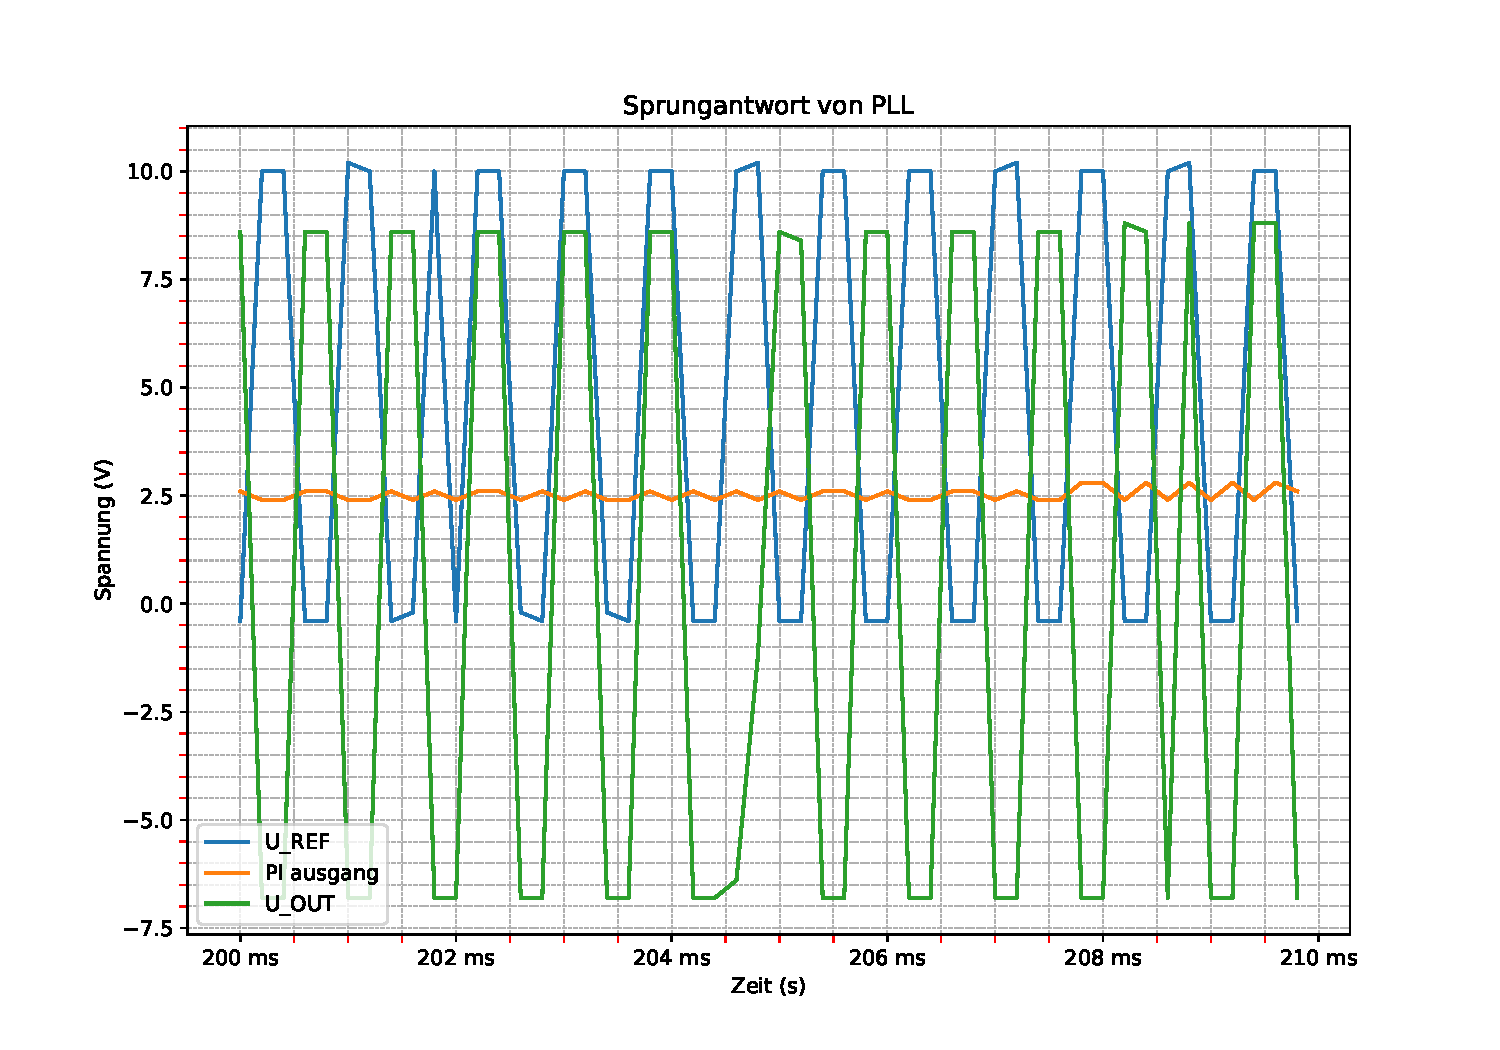
\includegraphics[width=0.8\linewidth]{Elektronik-Laborprotokoll_PLL/Abbildungen/sprungantwort_zoom.pdf}
  \caption{Detailansicht der Oszillationen von des PLL Sprungantwort}
  \label{fig:spa_zoom}
\end{figure}
In der Detailansicht des Diagramms werden zwei Rechteckwellen gezeigt, die aufgrund hoher Frequenzen Abtastfehler aufweisen, wodurch die Kanten trapezförmig oder manchmal dreieckig erscheinen. Diese Darstellungsart resultiert aus den Abtastfehlern sowie der linearen Interpolation der Matplotlib-Bibliothek. Es wird deutlich, dass \(U_{REF}\) und \(U_{OUT}\) nahezu identische Frequenzen aufweisen, was die Effizienz des Phasenvergleichs und die Anpassungsfähigkeit des Systems unterstreicht. 

\begin{figure}[H]
  \centering
  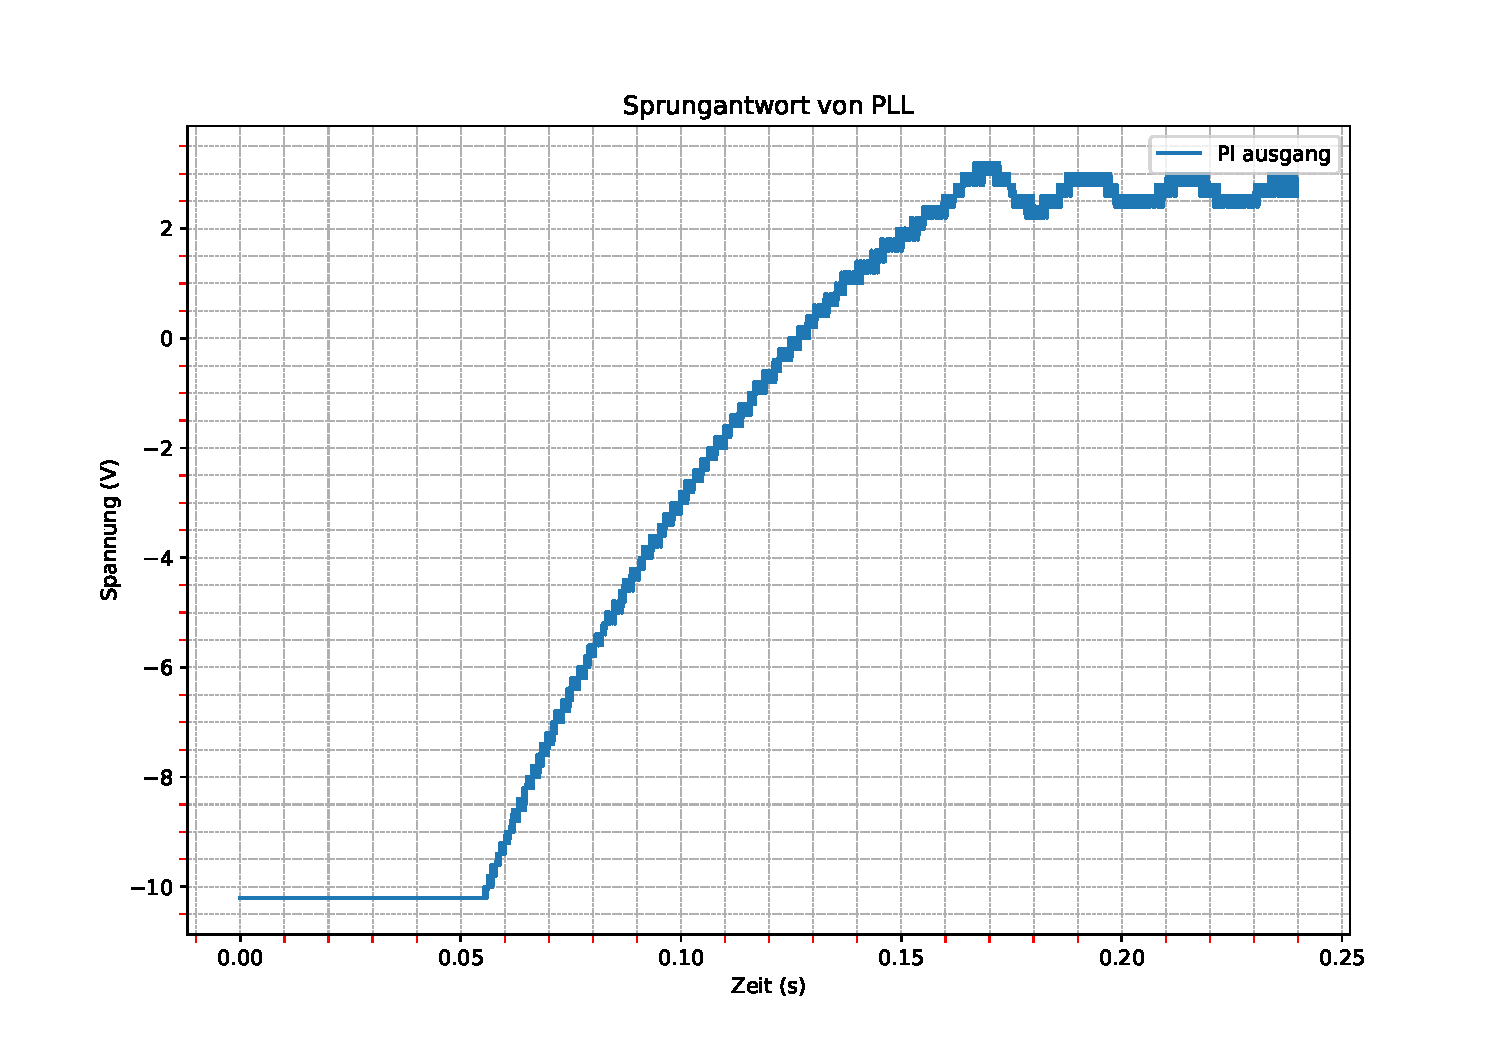
\includegraphics[width=0.8\linewidth]{Elektronik-Laborprotokoll_PLL/Abbildungen/sprungantwort.pdf}
  \caption{Vereinfachte Darstellung der Eingangsspannung des VCO-Komponenten im PLL-System.}
  \label{fig:spa}
\end{figure}

In der vereinfachten Darstellung wird ausschließlich die Eingangsspannung des spannungsgesteuerten Oszillators (VCO) gezeigt, welche dem Ausgangssignal des PI-Filters entspricht. Diese Fokussierung auf die VCO-Eingangsspannung ermöglicht eine klarere Analyse des dynamischen Verhaltens des PLL-Systems. Aus dem Diagramm lässt sich eine Periodendauer der Überschwingungen von etwa \SI{20}{\milli\second} ablesen. Dies entspricht einer Eigenfrequenz \(\omega_n\) von:
\[
\omega_n = \frac{2\pi}{T} = 2\pi \cdot \SI{50}{\hertz}= \frac{2\pi}{\SI{20}{\milli\second}} \approx \SI{314}{\radian\per\second} \text{ oder } f_n \approx \SI{50}{\hertz}
\]

Das Schleifenfilter wurde so dimensioniert, so dass $\omega_n$  $2\pi \cdot \SI{20}{\hertz}$ betragen würde. Es handelt sich um schon eine massive Abweichung von dem Soll-Wert, trotzdem kann diese Abweichung nur mit Messfehlern oder mit dem Effekt der unerwünschten realen Eigenschaften aller Bauteile, die für PLL verwendet wurde erklärt werden.

Wir sehen, dass die Sprungantwort einige Überschwingung hat, es ist Unterdämpft, Jedoch sind die Überschwingung klein, können wir schätzen $\frac{1}{2}<\delta<1$ als Dämpfungsfaktor. Was auch stimmt mit dem verwendeten Sollwert, mit dem die restliche Schaltung dimensioniert wurde und der $\delta=0.7$ beträgt, dafür überein.
%Der Dämpfungsgrad \(\delta\) kann aus der Peak-to-Peak-Amplitude der aufeinanderfolgenden Überschwingungen abgeschätzt werden. Wenn die initiale Überschwingung eine Amplitude von etwa \SI{1}{\volt} hat und die darauffolgende einen Abstand von \SI{1}{\volt} Peak-to-Peak aufweist, entspricht dies einem Dämpfungsgrad von \(\delta \approx 1\).
%FRAGE: IST D der DAMPFUNGSFANKTOR???? WIRKLICH??? 
%Da oben ist bullshit von tutor, schrebe es um


\begin{figure}[H]
  \centering
  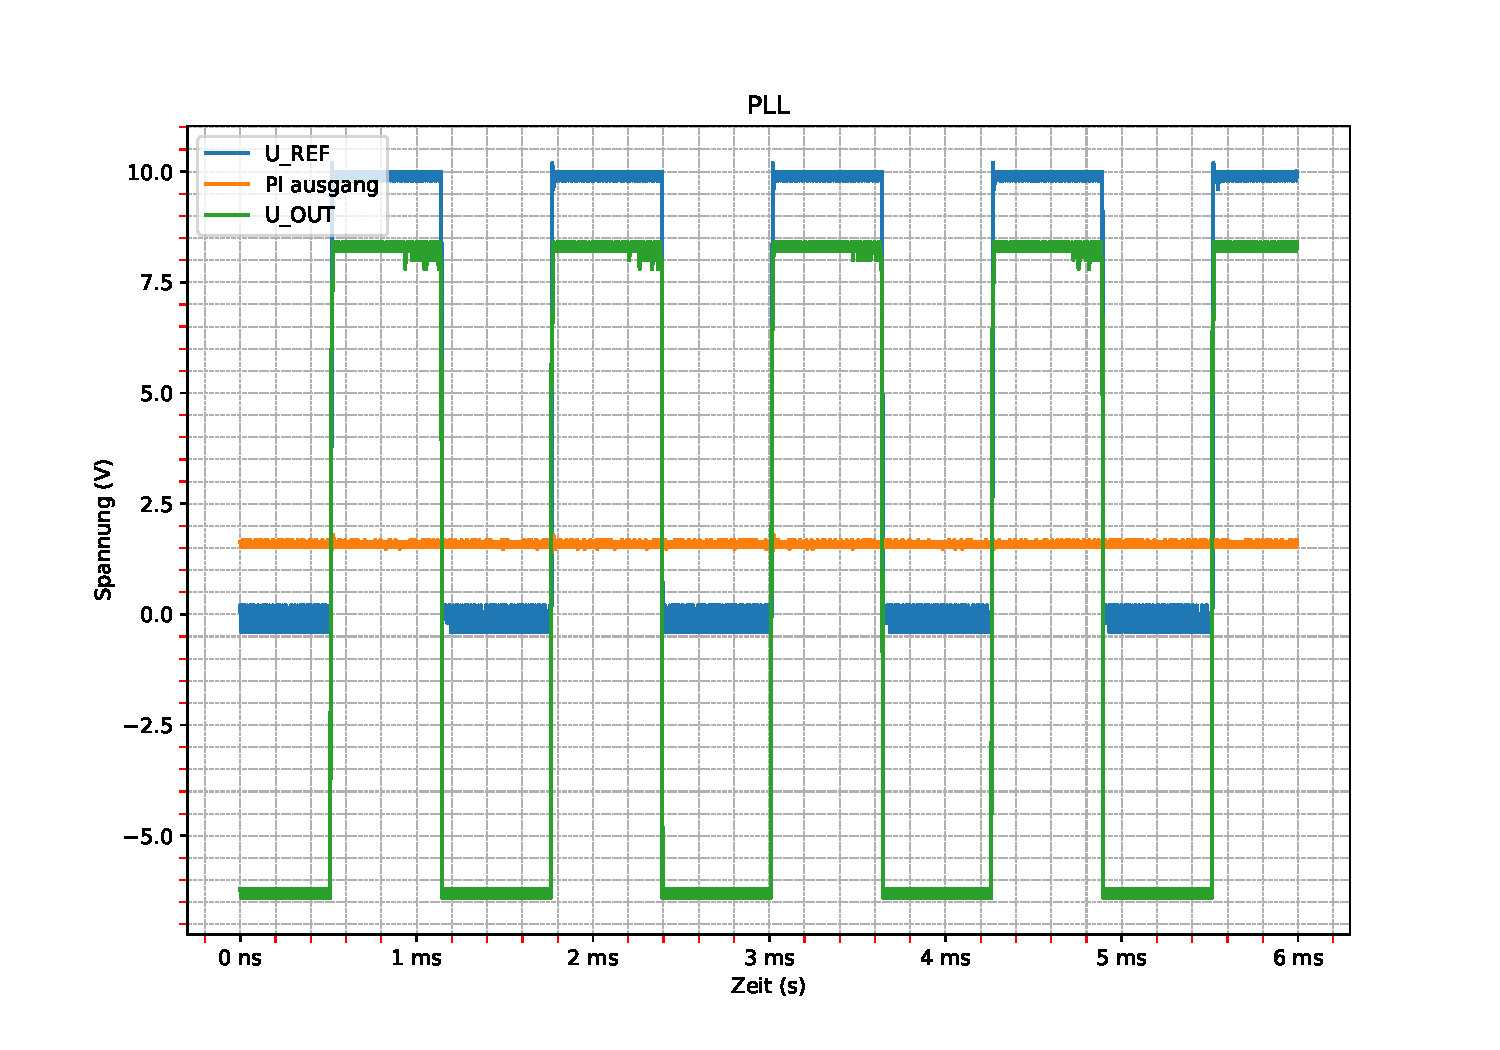
\includegraphics[width=0.8\linewidth]{Elektronik-Laborprotokoll_PLL/Plots/PLL_gemessen.pdf}
  \caption{gemessen PLL-final}
  \label{fig:PLL_alles_gemessen}
\end{figure}

In der folgenden Abbildung \ref{fig:eingerastet} ist der eingerastete der ausgerastete Zustand der simulierten PLL dargestellt.

\begin{figure}[H]
  \centering
  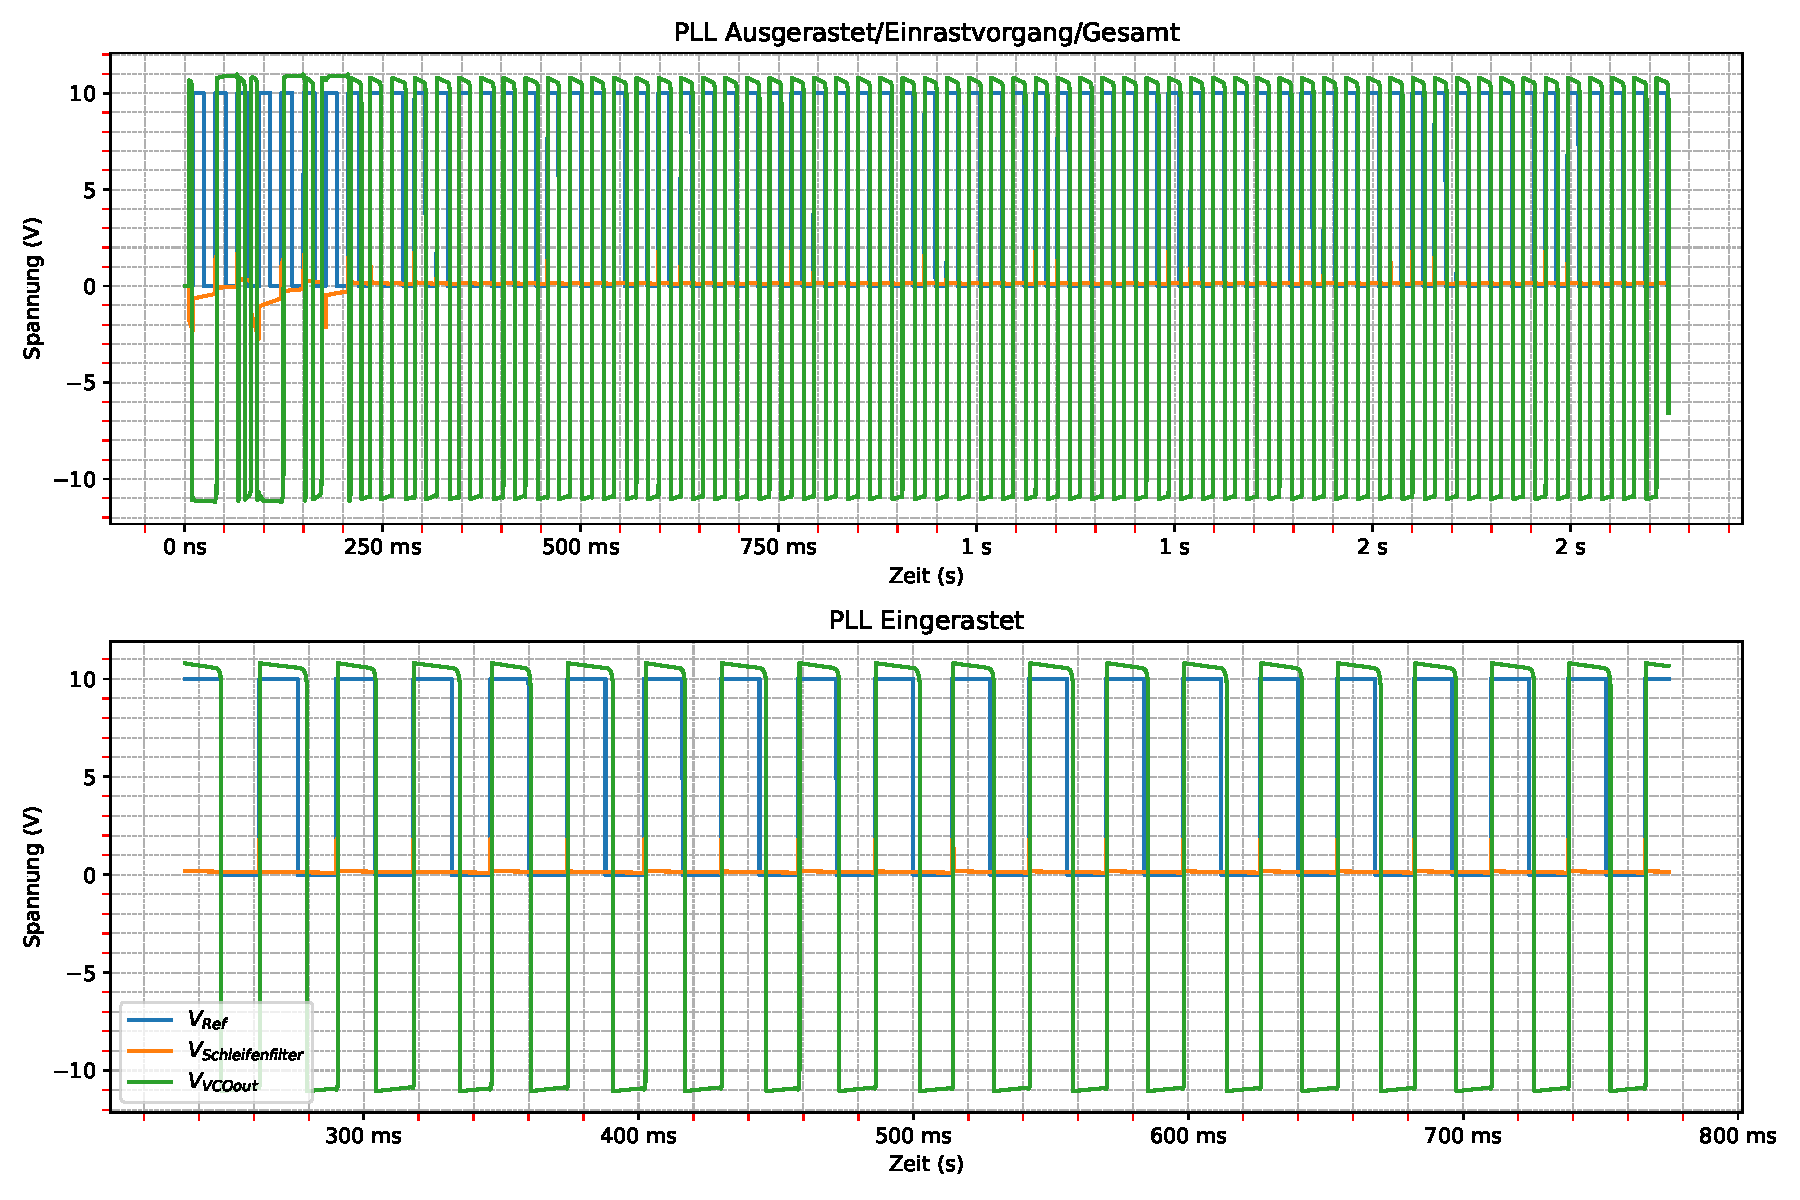
\includegraphics[width=0.8\linewidth]{Elektronik-Laborprotokoll_PLL/Plots/PLL-eingerastet.pdf}
  \caption{eingerastet und ausgerastet}
  \label{fig:eingerastet}
\end{figure}


Im Allgemeinen weisen die Graphen der PLL-Schaltung in der Simulation viele Ähnlichkeiten wie der in dem Labor aufgebauten Schaltung auf. Obwohl die Versorgungsspannung \SI{-12}{\volt} und \SI{12}{\volt} beträgt, werden diese Spitzenwerte weder in der gemessenen Schaltung noch in der simulierten Schaltung wegen Verlusten erreicht. Im Vergleich zur im Labor aufgebauten Schaltung beginnt die Oszillation in der Simulation viel schneller. 